% arara: xelatex
% arara: xelatex
% arara: xelatex


% options:
% thesis=B bachelor's thesis
% thesis=M master's thesis
% czech thesis in Czech language
% english thesis in English language
% hidelinks remove colour boxes around hyperlinks

\documentclass[thesis=B,english]{FITthesis}[2012/10/20]

% \usepackage[utf8]{inputenc} % LaTeX source encoded as UTF-8
% \usepackage[latin2]{inputenc} % LaTeX source encoded as ISO-8859-2
% \usepackage[cp1250]{inputenc} % LaTeX source encoded as Windows-1250

\usepackage{graphicx} %graphics files inclusion
\usepackage{float}
\usepackage{csquotes}
% \usepackage{subfig} %subfigures
% \usepackage{amsmath} %advanced maths
% \usepackage{amssymb} %additional math symbols
\usepackage{dirtree} %directory tree visualisation
\usepackage{subcaption}

\usepackage[dvipsnames]{xcolor}
\usepackage{listings}
\usepackage{titlesec}


\lstdefinelanguage{Kotlin}{
  comment=[l]{//},
  commentstyle={\color{gray}\ttfamily},
  emph={delegate, filter, first, firstOrNull, forEach, lazy, map, mapNotNull, println, return@},
  emphstyle={\color{OrangeRed}},
  identifierstyle=\color{black},
  keywords={abstract, actual, as, as?, break, by, class, companion, continue, data, do, dynamic, else, enum, expect, false, final, for, fun, get, if, import, in, interface, internal, is, null, object, override, package, private, public, return, set, super, suspend, this, throw, true, try, typealias, val, var, vararg, when, where, while},
  keywordstyle={\color{NavyBlue}\bfseries},
  morecomment=[s]{/*}{*/},
  morestring=[b]",
  morestring=[s]{"""*}{*"""},
  ndkeywords={@Deprecated, @JvmField, @JvmName, @JvmOverloads, @JvmStatic, @JvmSynthetic, Array, Byte, Double, Float, Int, Integer, Iterable, Long, Runnable, Short, String},
  ndkeywordstyle={\color{BurntOrange}\bfseries},
  sensitive=true,
  stringstyle={\color{ForestGreen}\ttfamily},
}


% % list of acronyms
% \usepackage[acronym,nonumberlist,toc,numberedsection=autolabel]{glossaries}
% \iflanguage{czech}{\renewcommand*{\acronymname}{Seznam pou{\v z}it{\' y}ch zkratek}}{}
% \makeglossaries

% % % % % % % % % % % % % % % % % % % % % % % % % % % % % % 
% EDIT THIS
% % % % % % % % % % % % % % % % % % % % % % % % % % % % % % 



\department{Department of Software Engeeniring}
\title{StudyPad - Android Client}
\newcommand{\appname}{StudyPad}

\newcommand{\innersection}[1]{\textbf{#1}}


\newcommand{\present}{\begin{minipage}{.1\textwidth}
\centering
      
\includegraphics[width=15pt, height=15pt]{ic_star_black_24dp}
    \end{minipage}}
    
\newcommand{\limited}{\begin{minipage}{.1\textwidth}
\centering
      
\includegraphics[width=15pt, height=15pt]{ic_star_half_black_24dp}
    \end{minipage}}
    
    
\newcommand{\absent}{\begin{minipage}{.1\textwidth}
\centering
      
\includegraphics[width=15pt, height=15pt]{ic_star_border_black_24dp}
    \end{minipage}}
    
\newcommand{\quoting}[1]{\textit{``#1"}}
\newcommand{\fullStar}
	{\begin{figure}[H]
	\centering
  
\includegraphics[scale=0.1]{ic_star_black_24dp.png}
\end{figure}}





\authorGN{Roman} %author's given name/names
\authorFN{Levinzon} %author's surname
\author{Roman Levinzon} %author's name without academic degrees
\authorWithDegrees{Roman Levinzon} %author's name with academic degrees
\supervisor{Ing. Miroslav Bal{\'i}k, Ph.D}
\acknowledgements{First and foremost, I would like to thank my supervisor Ing. Miroslav Bal{\'i}k, Ph.D for his patience, understanding, support and valuable advices during the whole process of writing this thesis.

I also would like to take this opportunity to thank my family for their support
during the whole period of my study.}
\abstractEN{StudyPad is a combination of a note-taking service and a social network, aimed at helping students to memorise different pieces of information.  The goal of this thesis is to develop an application for Android OS that will serve as the client. This text acknowledges existing solutions, contains domain and requirements analysis, description and the choice of application's architecture its implementation and testing.}


\abstractCS{StudyPad je kombinace slu{\v z}by pro po{\v r}izov{\'a}n{\' i} pozn{\'a}mek a soc{\'i}{\'a}ln{\'i} s{\'i}t{\v e} s c{\'i}lem  pomoci student{\r u}m zapamatovat si r{\r u}zn{\'e} informace. C{\'i}lem pr{\'a}ce je vyvinout aplikaci pro OS Android, kter{\'a} bude slou{\v z}it jako klient. Tento text uv{\'a}d{\' i} p{\v r}ehled st{\'a}vaj{\' i}c{\'i}ch {\v r}e{\v s}en{\'i}, obsahuje anal{\'y}zu dom{\'e}ny a po{\v z}adavku, popis a v{\'y}b{\v e}r architektury aplikace, jej{\'i} implementace a testov{\' a}n{\' i}}
\placeForDeclarationOfAuthenticity{Prague}
\keywordsCS{Mobiln� aplikace, Android, Kotlin, MVVM, Clean architecture, vzd{\v e}l�v�n�}
\keywordsEN{Mobile application, Android, Kotlin, MVVM, Clean architecture, education}
\declarationOfAuthenticityOption{1} %select as appropriate, according to the desired license (integer 1-6)
% \website{http://site.example/thesis} %optional thesis URL


\begin{document}

% \newacronym{CVUT}{{\v C}VUT}{{\v C}esk{\' e} vysok{\' e} u{\v c}en{\' i} technick{\' e} v Praze}
% \newacronym{FIT}{FIT}{Fakulta informa{\v c}n{\' i}ch technologi{\' i}}

\setsecnumdepth{part}
\chapter{Introduction}

Each year, our smartphones get smarter and mobile applications become more advanced. The arrival of smartphones and mobile applications has completely changed our way of living, made it easier, and it is hard to come up with a single aspect of life, that has not been improved by one or the other application. They are everywhere: helping us to navigate in our neighbourhood, keeping us up to date with latest news, helping us to stay in touch with our loved ones, stay fit and healthy and more. In addition, some of the most popular applications tend to teach us something new.

Educational applications are very popular on both most popular mobile platforms (iOS and Android). Many of them use a flash card system in the study process -- displaying small pieces of information one after another, so that the user can memorise it more efficiently. However, most of these services are fairly limited in terms of what they are trying to teach and some of the greatest  features are scattered across different applications and services. \appname\ is a new solution to this problem. Using Android OS, today's most popular mobile platform, \appname\ wants to give its users freedom in what they can learn and give them proper tools to share, exchange and collaborate on study materials to make the education process even more easier.

\section{Goal}
The goal of this thesis is to deliver  \appname\ client application for  Android OS with the emphasis on content creation, sharing and collaboration. This includes following steps:
\begin{itemize}
	\item analysis of  the existing solutions,
	\item analysis of the functional and non-functional requirements,
	\item requirements design and its implementation,
	\item testing of the resulted solution.
\end{itemize}

\section{Motivation}

The primary motivation is to practice software
development processes on the big and scalable project while applying advanced practices and technics of Android Development. 

\setsecnumdepth{all}

\chapter{State-of-the-art}
This chapter serves as an introduction of what StudyPad is trying to achieve and compares it to the other applications and services available.  In order to make this comparison more detailed, functional and non-functional requirements are established here.

\section{StudyPad Service}
\appname\ is a combination of a note-taking service and a social network. It is intended for students and everyone who wishes to learn something new. The primary focus of this version of  \appname\ is on content creation, its sharing and discovery. 


Currently \appname\ service consists of four components and each and every one of them originated from several subjects on Faculty of Information Technology (FIT) in Czech Technical University (CTU). I have developed the very first iteration of the backend service as a semestral project for subject Enterprise Java (BI-EJA). Another subject, Programming for the Android Operating System (BI-AND), taught me the basics of the Android Development which then resulted in developing the first Android prototype. Recently added iOS client is the output of my semestral project for subject Fundamentals of iOS Application Development for iPhone and iPad (BI-IOS). Most important components will be described more thoroughly in Chapter 2.

\begin{figure}[H]
\centering
  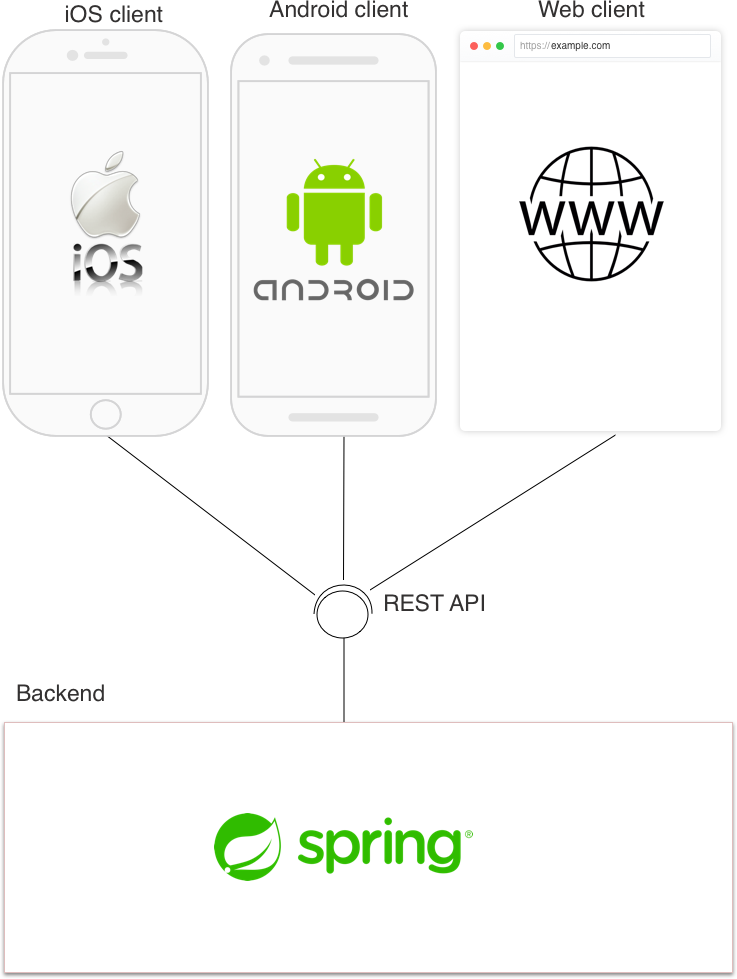
\includegraphics[scale=0.25]{systemdesc}
  \caption{\appname\ Sevice}
  \label{fig:android-component}
\end{figure}




\appname\ core concepts are \textit{Notebooks} and \textit{Notes}. The notebook is simply a collection of notes united by one theme. This may be a subject in school, a language that you would like to learn or a set of questions that you could hear at a job interview. Note, in turn, is a part of the notebook and represents a single piece of information that has a name and a content. It can also be interpreted as a question and answer or a term and its definition.


Each user has his/her own space where they can create, store and edit notebooks and notes (hereafter \textit{Library}). All notebooks stored in the library can be used in various tests and exercises to help users to memorise its content.


\subsection{Sharing \& Collaboration}

\appname\ also allows users to share their notebooks with each other easily. Each notebook can be shared by creating a published version of it (hereafter Published Notebook), thereby making it available to everyone else for viewing and importing.
The publication process involves providing additional information about the notebook, including its name, an optional description, topic and set of optional tags to narrow the topic. Everything the user has provided along with their school and language will then be used in the process of searching and filtering -- which will facilitate the search for the necessary materials. \appname\ also makes it possible to quickly share a notebook by sending a link, which will act as a deep-link, navigating the user directly to a Published Notebook.

The user that has initially published the notebook (hereafter \textit{Author}) reserves the right to make edits/corrections to the Published Notebook. Other users (hereinafter \textit{Subscribers}) in turn can save a Published Notebook to their library and suggest some changes or corrections to improve the content. By saving Published Notebook to his/her library, the subscriber will be able to make any local changes as he/she sees fit, which later can be made into Suggestions. The Subscriber will be notified about any updates made to the Published Notebook so that he/she can apply the changes to his/her local version, in case of conflicts Published version will be used. The Author of the notebook, in turn, will be notified about the latest suggestions and comments left by the subscribers.




\section{Requirements}
It is important to establish all functional and non-functional requirements for \appname. The section bellow contains all requirements designated  before the start of the development.

\subsection{Functional Requirements}
\bigskip
\textbf{User Authentication}
\begin{itemize}
	\item \textbf{F1: Registration/Login using email} Access to \appname\ will be possible by creating an account using an email address/password combination.
	\item \textbf{F2: Registration/Login using Facebook} The user will be able to use his/her Facebook account to access \appname.
	\item \textbf{F3: Registration/Login using Google} The user will be able to use his/her Google account to access \appname.
	\item \textbf{F4: Store OAuth token} API Authentication Token will be stored in a device memory.
	\item \textbf{F5: Token refreshment} API Token will be refreshed when needed, so the user will not have to login again.
	\item \textbf{F6: University selection} As part of user registration flow, the user will be able to select his/her university.
	\item \textbf{F7: University Addition} The user will be able to add his/her school, in case of not finding it in a \appname\ database.
\end{itemize}
\bigskip
\newpage
\textbf{Library Management (Notes \& Notebooks)}
\begin{itemize}
	\item \textbf{F8: Notebook creation} The user will be able to create new notebooks with the name he/she choose.
	\item \textbf{F9: Notebook deletion} The user will be able to delete existing notebooks.
	\item \textbf{F10: Notebook name edition} The user will be able to edit notebooks names.
	\item \textbf{F11: Note creation} The user will be able to create a note with a specific title and content.
	\item \textbf{F12: Note edition} The user will be able to edit an existing note, or completely delete it.
	\item \textbf{F13: Show Notebooks} The user will be able to view all the notebooks he/she created.
	\item \textbf{F14: Show Notes} By clicking on notebook item, the user will be able to view the list of notes that are assigned to this notebook.
	\item \textbf{F15: Mathematical Expressions Support} User will be able to use complex mathematical expressions as notes content.
\end{itemize}

\bigskip
\textbf{Sharing Hub}
\begin{itemize}
	\item \textbf{F16: View published notebooks} The user will be able to view notebooks published by other users.
	\item \textbf{F17: Search through published books} The user will be able to search through the published notebooks by applying different filters (such as author, university, and subject/topic).
	\item \textbf{F18: Browse through published notebook} User will be able to see notes inside the notebook that has been published.
	\item \textbf{F19: View comments} User will be able to view others users comments discussing a notebook that have been published.
	\item \textbf{F20: Leave a comment} The user can comment on an other user published notebook.
	\item \textbf{F21: Delete a comment} The application will allow the user to delete his/her comment.
	\item \textbf{F22: Edit a Comment} The application will allow the user to edit his/her comment.
	\item \textbf{F23: Save published notebook} User will be able to save published notebook to his/her library.
	\item \textbf{F24: Publish notebook} User will be able to publish his/her notebook.
	\item \textbf{F25: Update published notebook} The Author of the published notebook will be able to update its information.
		\item \textbf{F26: Share notebook} The user will be able to share his/her notebook by generating a deep-link.
	\item \textbf{F27: Notification on update} The user will be notified on updates to the Published notebook they have subscribed to.
	\item \textbf{F28: Suggestions} Subscribers will be able to suggest a change or correction to the Published Notebook.
	\item \textbf{F29: Suggestions Review}  The author will be able to approve the suggestions, which will result in the update of the Published Notebook, or reject it.
	\item \textbf{F30: Copy Published Notebook} The user will be able to copy a published notebook. This will create a standalone copy of this notebook in the user's library.
 \end{itemize}

\bigskip
\textbf{Challenges}
\begin{itemize}
	\item \textbf{F31: Start a Flashcards walkthrough} The user will be able to use an interactive method of looking through his/her notes.
	\item \textbf{F32: Start a written test} The user will be able to participate in a written test based on one of the notebooks to test his/her knowledge.
	\item \textbf{F33: Start a self-check} The user will be able to participate in a self-check challenge that will be based on one of his/her notebooks.
	
\end{itemize}


\bigskip
\textbf{Profile}
\begin{itemize}
	\item \textbf{F34: View Profile Information} The user will be able to view his/her profile information such as first name, last name, and  university.
	\item \textbf{F35: Edit Profile Information} The user will be able to edit his/her profile information.
	\item \textbf{F36: Logout} The user will be able to logout from the application.
\end{itemize}


\subsection{Non-functional requirements}

\begin{itemize}
  \item \textbf{N1: Native Android application}  The application will be written using native Android SDK.
  \item \textbf{N2: Android Version} The application minimal SDK version must be low enough to support as many devices as possible and high enough to use most applicable  Android APIs considering other functional and non-functional requirements.
  \item \textbf{N3: Material Design} The application user interface will follow the latest Material design guidelines and best practices.
  \item \textbf{N4: Scalable app architecture} The application's architecture must be scalable and easy testable.
    \item \textbf{N5: App Localisation} The application will be able to adapt to different languages based on user locale.
\end{itemize}


\newpage

\section{Existing solutions}

There are several services out there whose goal is similar to \appname. However, most of those solutions are specialised in language-learning and have limited sharing and/or searching options. Each application/service will be reviewed separately and will include a requirements and main processes comparison. 

Symbols are used in Tables  to indicate  requirement availability in the applications. The symbol in Figure \ref{fig:star} represents the functionality  that is fully supported by the application. The symbol in Figure \ref{fig:starhalf} demonstrates that the given functionality is either limited/incomplete or not working as intended. Lastly, symbol in Figure \ref{fig:starborder} indicates that the given application does not support the requirement.
 
\begin{figure}[H]
\centering
\begin{subfigure}{.3\textwidth}
  \centering
  
\includegraphics[scale=0.28]{ic_star_black_24dp}
  \caption{Present Feature}
  \label{fig:star}
\end{subfigure}%
\begin{subfigure}{.3\textwidth}
  \centering
  
\includegraphics[scale=0.2]{ic_star_half_black_24dp.png}
  \caption{Limited Feature}
  \label{fig:starhalf}
\end{subfigure}%
\begin{subfigure}{.3\textwidth}
  \centering
  
\includegraphics[scale=0.2]{ic_star_border_black_24dp.png}
  \caption{Absent Feature}
  \label{fig:starborder}
\end{subfigure}

\end{figure}



\subsection{StudyBlue}

\textbf{StudyBlue} not only partially shares a name with \appname\ but also a goal and a wide range of features. It is clearly one of the biggest rivals on the market and it is very important to determine what StudyBlue does right and what it does not. How most important \appname\ requirements are compared to the StudyBlue functionality can be seen on Table \ref{tab:studyblue}.

Notebooks here are called \textit{decks} and notes are represented by \textit{cards}. Moreover, all decks in StudyBlue are stored in specialised folders named Classes and Interests. Interest, as an entity, not only stores decks, but also unites them by a subject or a topic (e.g. Spanish, Literature). Being a student of the university, the user can also create an Interest that will be connected to his/her school -- Class. Both Interests and Classes are split into two parts: shared space, where the user can find all the decks created by other users, and personal space, where the user can keep the decks he/she has created, saved or copied.


\begin{table}[H]
\centering
\caption{\appname\ \& StudyBlue requirements comparison}
\label{tab:studyblue}
\begin{tabular}{|l|c|c|}
\hline
\multicolumn{1}{|c|}{\textbf{Requirements / Application name}} & \multicolumn{1}{l|}{\textbf{StudyPad}} & \multicolumn{1}{l|}{\textbf{StudyBlue}} \\ \hline
F6: University Selection                                       & \present                                & \present                                \\ \hline
F14: Show Notes                                                & \present                              & \limited                                \\ \hline
F15: Mathematical Expressions Support                              & \present                               & \limited                                \\ \hline
F16: Browse Published Notebooks                        & \present                                & \present                               \\ \hline
F17: Searching For Published Notebooks                    & \present                                & \present                               \\ \hline
F19-F22: User Commentaries                                     & \present                                & \absent                                \\ \hline
F28-F28: User Suggestions                                          & \present                                & \absent                               \\ \hline
\end{tabular}
\end{table}

\begin{itemize}
	\item \textbf{Library management:} The main difference in library management comes with the fact that each deck must be associated with an Interest or Class, moreover, it is not possible just to create a deck, the user has to create at least two cards first. Because of that, library management not only includes managing your decks and cards, but also interests and classes. Everything the user has saved or created, whether class, interest or a deck can be accessed via \textit{Backpack} -- User's personal library.
	\item \textbf{Publishing:} The Publishing process is quite different compared  to what \appname\ is trying to achieve. When creating a deck, the user can choose whether they want to make his/her deck visible for other users in this Class/Interest or to make it private. It is not possible to collaborate on a deck or suggest a change.
	
	\item \textbf{Importing}: As mentioned before, user can save a deck from an existing Interest/Class to their personal space, but they will not be able to make any edits without making a copy.
	\item \textbf{Discovering:} The fact that all decks are either assigned to an Interest or a Class makes searching quite simple. The user can search for deck, classes and users by its name. All these searching options are separated in the UI, so there is no way of combining them. Searching based on the Interest is also available, but the user has to add this Interest to his/her Backpack.
	\item \textbf{UI \&  UX}: StudyBlue has been in development roughly since 2009, and as for now, UI looks outdated and UX can be greatly improved. The most common UI issue here -- Inconsistent usage of UI elements styles.
\end{itemize}

 \subsection{Quizlet}
\textbf{Quizlet} is primarily used for learning languages, from where most of the limitations come from. The closest analogy to a Notebook here is a Study set with Terms inside. Being an application for language learners makes the process of generating different tests and quizzes quite easy, and this is where this application shines the most. Table \ref{tab:quizlet} shows requirements comparison between \appname\ and Quizlet.

\begin{table}[H]
\centering
\caption{\appname\ \& Quizlet requirements comparison}
\label{tab:quizlet}
\begin{tabular}{|l|c|c|}
\hline
\multicolumn{1}{|c|}{\textbf{Requirements / Application name}} & \multicolumn{1}{l|}{\textbf{StudyPad}} & \multicolumn{1}{l|}{\textbf{Quizlet}} \\ \hline
F6: University Selection                                       & \present                                & \absent                                \\ \hline
F14: Show Notes                                                & \present                                                                & \limited                                \\ \hline
F15: Mathematical Expressions Support                               & \present                                                                & \absent                                \\ \hline
F16: Browse Published Notebooks                         & \present                                                                & \present                               \\ \hline
F17: Search For Published Notebooks                    & \present                                                                & \limited                               \\ \hline
F19-F22: User Commentaries                                    & \present                                                                & \absent                                \\ \hline
F28-F28: User Suggestions                                           & \present                                                                & \limited                               \\ \hline
\end{tabular}
\end{table}

\begin{itemize}
	\item \textbf{Publishing}: Similar to StudyBlue, all Study Sets are visible to everyone else by default. However, Quizlet provides a wider variety of privacy options. Study Set can either be completely public, private or semi-private using a password protection. Password protection can also be used to allow certain users to modify a study set.
	\item \textbf{Importing}: Importing flow allows user to either copy or save the study set to a specific folder. This flow may confuse some users, because only copy allows the user to actually add a study set to their library and modify it. Saving study set to the specific folder only saves the link to it and splits library management in two parts.
	\item \textbf{Discovering:} This limitation comes from the fact that Quizlet is an app for studying foreign  languages. As a consequence, the only distinctions between Study Sets are its name and its language. These are the only two options available when searching through study sets.

\end{itemize}

\subsection{Cram}
\textbf{Cram} is very similar to Quizlet but seems highly outdated in terms of UX/UI and brings some sharing limitations to the table. Table \ref{tab:cram} shows a requirements comparison between \appname\ and Cram.



\begin{table}[H]
\centering
\caption{\appname\ \& Cram requirements comparison}
\label{tab:cram}
\begin{tabular}{|l|c|c|}
\hline
\multicolumn{1}{|c|}{\textbf{Requirements / Application name}} & \multicolumn{1}{l|}{\textbf{StudyPad}} & \multicolumn{1}{l|}{\textbf{Cram}} \\ \hline
F6: University Selection                                       & \present                                & \absent                             \\ \hline
F14: Show Notes                                                & \present                                & \present                            \\ \hline
F15: Mathematical Expressions Support                            & \present                                & \limited                            \\ \hline
F16: Browse Through Published Notebooks                        & \present                                & \present                            \\ \hline
F17: Search For Published Notebooks                    & \present                                & \limited                            \\ \hline
F19-F22: User Commentaries                                     & \present                                & \absent                             \\ \hline
F28-F28: User Suggestions                                          & \present                                & \absent                             \\ \hline
\end{tabular}
\end{table}

\begin{itemize}
	\item  \textbf{Publishing:} Content publishing is similar to Quizlet -- All sets are either visible by other users or not. Sharing a deep-link to a single study set was not functional at the time of writing this section.
	\item \textbf{Discovering}: Searching for content in Cram is even more limited compared to Quizlet, only the name of the study set is used.
	\item \textbf{Importing}: Library management here is split in three parts: User personal sets, Favourite sets and Recently studied. When searching, there is no way to save a published study set to a personal library, however, it will be automatically saved to Recent section, or the user can add it manually to Favourites. It is not possible to make any local edits.
\end{itemize}


\subsection{TinyCards}

\textbf{TinyCards} is a flash-card application made the same developer that created Duolingo --  one of the biggest language-learning applications on the market. TinyCard is meant to be more generic as it alows users to create custom study sets, often not limited to languages. Table \ref{tab:tinycards} shows how the \appname\ requirements compare to the TinyCards functionalities.

\begin{table}[H]
\centering
\caption{\appname\ \& TinyPads requirements comparison}
\label{tab:tinycards}
\begin{tabular}{|l|c|c|}
\hline
\multicolumn{1}{|c|}{\textbf{Requirements / Application name}} & \multicolumn{1}{l|}{\textbf{StudyPad}} & \multicolumn{1}{l|}{\textbf{TinyCards}} \\ \hline
F6: University Selection                                       & \present                                & \absent                                  \\ \hline
F13: Show Notes                                                & \present                                & \present                                 \\ \hline
F14: MathJax /ASCII Math support                               & \present                                & \absent                                  \\ \hline
F16: Browse Through Published Notebooks                        & \present                                & \present                                 \\ \hline
F17: Search Through Published Notebooks                    & \present                                & \limited                                 \\ \hline
F18-F21: User Commentaries                                     & \present                                & \absent                                  \\ \hline
F27: User Suggestions                                          & \present                                & \absent                                  \\ \hline
\end{tabular}
\end{table}


	\begin{itemize}
		\item \textbf{Importing:} Similar to Cram, it is not possible to edit the study set the user has downloaded and saved to their library.
		\item \textbf{Challenges:} Tests are generated automatically and there is no way to choose the test type.
	\end{itemize}






\chapter{Analysis}
This chapter serves as an introduction to Android development and gives an overview of the core technologies and tools used. Also, it provides a domain and requirements analysis and overall system description.

\section{Android Platform}
Android is a mobile operating system developed by Google. It is based on a modified version of the Linux kernel and other open source software, and is designed primarily for touchscreen mobile devices such as smartphones and tablets\cite{android-platform}.



\subsection{Android SDK Versions}
Since its inception, several versions have been released, with the latest one  (by the time of writing this thesis) being 9.0, codenamed \enquote{Pie}. Every new version provides new and improved APIs to work with and backward compatibility for applications running on older versions\cite{android-sdks}. Originally, the Support Libraries were used to provide backward compatibility while targeting newer versions. This was the case until AndroidX was introduced.

AndroidX, in essence, is a refactored version of the Support Libraries. Just like Support Libraries it ensures backward-compatibility and is shipped separately from the Android OS. Additionally, it provides more clear and convenient package names and uses a strict semantic versioning system\cite{androix-overview}.

When developing applications for Android, the developer has to consider which OS versions the application will support. Specifically, the \texttt{minSdkVersion} and \texttt{targetSdkVersion} attributes are used to identify the lowest API level with which your application is compatible and the highest API level against which you have designed and tested your application. 

\newpage \noindent \appname\ will target the latest Android version available, with the minimal version set to 5.0, codenamed Android Lollipop. This will ensure a high compatibility rate of 89\% and Material Design Support, which is one of the non-functional requirements.


\begin{figure}[H]
\center
  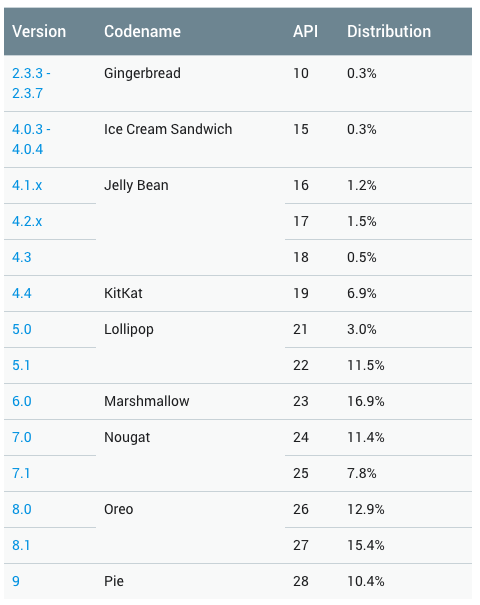
\includegraphics[scale=0.5]{androidversion.png}
  \caption{Android Versions distribution\cite{android-distribution}}
  \label{fig:androidversions}
\end{figure}

\subsection{Android High-level Framework Elements}
Android SDK provides multiple elements and APIs for developers to help them build their applications.
\begin{itemize}
	\item \textbf{Activity}: \texttt{Activity} represents a single window where the UI elements can be placed. Android OS managing the creation and destruction of the \texttt{Activities}, that is why \texttt{Intents} are used to start/launch them\cite{android-activity}. 
	\item \textbf{Fragment}: \texttt{Fragments} were introduced in Android 3.0, primarily to support more flexible UI designs for larger screens (like Tablets). In such designs, \texttt{Activity} serves as container for one or more \texttt{Fragments}, and because each \texttt{Fragment} defines its own layout with its own lifecycle, it can be used in multiple  \texttt{Activities}\cite{android-fragment}.
	\item \textbf{Broadcast Receiver}: \texttt{Broadcast Receiver} allows the application to receive and send local and system-wide broadcasts similar to the publish-subscribe design pattern. By using \texttt{Broadcast Receiver} application can act upon receiving various kind of events, like the change of internet connectivity or charging status\cite{android-br}.
	\item \textbf{Service}: \texttt{Service} is the application component that does not require UI and is used to perform long-running operations, even if the user stops interacting with the application\cite{android-service}.
	\item \textbf{Intent}: \quoting{An intent is an abstract description of an operation to be performed}. \texttt{Intent} can be used to launch an \texttt{Activity}, start a \texttt{Service} or a \texttt{BroadcastReceiver}. \texttt{Intent} can either start a specific component (explicit Intent) or try to find a component that can complete certain actions (implicit Intent)\cite{android-intent}. For example,  there could be several applications available on the device with the image viewing functionality, implicit intent, in this case, will allow the user to choose which application will handle this action. Explicit intent, on the other hand, is used to launch specific components using its class name.
	\end{itemize}
	
	
	\subsection{Resources}
Resources are the additional files and static content that your code uses, such as bitmaps, layout definitions, and user interface strings. Resources are stored in the separated package called \texttt{/res} and can be referenced in the application using ids. Also, depending on the current configuration, Android can choose appropriate resource version (if multiple are provided) at run-time. For example, it can be used for localisation support by providing different strings resources for different languages\cite{android-resources}.
	
	\subsection{Views} 
	
	\texttt{View} is a fundamental building block for all the UI components. It serves as a base class for \texttt{Widgets}, which are the interactive elements and \texttt{ViewGroups}, that acts as a container for other Views\cite{android-views}.     
    \texttt{ViewGroup}, as mentioned before, is an invisible container that holds other views. Android provides different ViewGroup subclasses, each with its own purpose and a way to structure its children\cite{android-viewgroup}. \texttt{LinearLayout}, for example, allows to align widgets horizontally or vertically\cite{android-linear}. Another important ViewGroup that has received a lot of attention and support during the last couple of years is ConstraintLayout. Using constraints allows the developer to create more complex layouts without using nested ViewGroups (i.e., LinearLayout inside another Linear Layout)\cite{android-constraints}.
    
    Android uses Extensible Markup Language (XML) for declaring the UI for Activities and Fragments. XML is then converted to the View object using \texttt{LayoutInfalter}.  Views can also be added programmatically via Java/Kotlin code.    

\section{Android Studio}
Android Studio is an official IDE for Android development. Out of the box it provides a lot of essential tools, like visual Layout editor, emulator and more.

\section{Gradle}
Gradle is a build toolkit, that is used to automate and manage the build process, while allowing you to define flexible custom build configurations using Groovy-based DSL (Domain Specific Language). Android plugin, shipped alongside the Android Studio, allows to modify and control various build parameters such as \texttt{buildVariant}, dependencies, artifacts signings, and manifest entries\cite{android-gradle}.

\section{Kotlin}
\quoting{Kotlin is a pragmatic programming language for JVM and Android that combines OO and functional features and is focused on interoperability, safety, clarity and tooling support.} Kotlin is a general purpose language developed by JetBrains and it works everywhere Java works and is fully interoperable with it, meaning every Java code can be converted to Kotlin and vice-versa\cite{kotlin}. Since May 17th 2018, Kotlin became the official language for Android development with all the tools and libraries required shipped with Android Studio out of the box\cite{kotlin-android}. 


\subsection{Kotlin Extensions}
Similar to some other languages, Kotlin provides a way to extend any class with new functionality without inheritance. There are two types of extensions: Functions and Properties. All the extensions are resolved statically and do not modify the class they extend\cite{kotlin-exts}.

When it comes to Android, a  plugin developed by JetBrains provides a lot of useful extensions that enhance the experience of Android development. For example, it is possible to reference Views from Activity/Fragments directly using its ids. Previously it was required to call \texttt{findViewById<View>()} (Listing \ref{code:viewbinding}) to obtain a view reference, which resulted in a lot of boiler-plate code\cite{kotlin-androidexts}.


 \begin{lstlisting}[caption={Kotlin View Binding example}, label={code:viewbinding}, language=Kotlin]
   // Instead of findViewById<TextView>(R.id.textView)
   textView.setText("Hello,world!")

\end{lstlisting}



Due to its official support and features, Kotlin was chosen as a primary language for \appname\ development as opposed to Java.

\section{Application Architecture}
Application Architecture defines the way different application elements interact with each other and how the application is designed and organised. This section aims to address different ways to approach the application architecture.

\subsection{Clean Architecture}
Clean architecture is a set of ideas derived from different kinds of other approaches with the main principle being the separation of concerns\cite{cleanarch}. 
Separation of concerns ensures that all the application's components are easily replaceable and as much independent as possible. When it comes to Android and every software that contains UI, it is essential that the UI does not contain any business logic and serves only as a way to show information.

 This approach will be used as the main guideline during application architecture design and implementation.


\subsection{MVP}
MVP or Model-View-Presenter is an architecture pattern that is very common in Android development. 
Model represents the data layer
View is the UI layer, which in the Android worlds are Fragments and Activities. 
Presenter -- is the layer between the View and the Model. It receives events from the View and updates the Model layer and applies the result to the UI layer.
The View and Presenter both are abstracted to Interfaces, thus making all the layers easily testable\cite{arch-mvp}. However, one of the main disadvantages is that Presenter must hold a reference to a View, which can lead to memory leaks and other problems around Android lifecycle.

\subsection{MVVM}
MVVM or Model-View-ViewModel is another pattern to apply Clean Architecture principles. It is very similar to MVP  when it comes to View and Model layers, with the only difference being ViewModel.
ViewModel, as oppose to Presenter, is not aware of the View -- it does not hold the reference to it. Instead, View subscribes to ViewModel events and updates its state accordingly. ViewModel handles UI interactions, updates the Model layer and then post changes so that the View can present these changes to the user\cite{arch-mvvm}.



\section{Firebase}

\quoting{Firebase lets you build more powerful, secure and scalable apps, using world-class infrastructure}\cite{firebase}. Firebase provides a high number of services, some of which are a necessity in today's world of software development. \\\appname\ will be using the following services:
\begin{itemize}
	\item \textbf{Firebase Analytics} Firebase Analytics provides free application measurement solution, that allows you analyse how the users interact with your application based  on up to 500 distinct events\cite{firebase-analytics}.
		\item \textbf{Firebase Cloud Messaging} \quoting{Firebase Cloud Messaging (FCM) provides a reliable and battery-efficient connection between your server and devices that allows you to deliver and receive messages and notifications on iOS, Android, and the web at no cost}\cite{firebase-messaging}.
	\item \textbf{Firebase Auth} \quoting{Firebase Auth  provides an end-to-end identity solution, supporting email and password accounts, phone auth, and Google, Twitter, Facebook, and GitHub login, and more}\cite{firebase-auth}.
	\item \textbf{Crashlytics} Crash Reporting allows you track detailed reports of the errors and crashes in the application. All the issues experienced by the users are then grouped into clusters of similar stack traces and triaged by the severity of impact on application users\cite{firebase-crash}.

\end{itemize}.

\noindent While Firebase Analytics and Crash Reporting services are a great help while developing mobile applications, Firebase Auth and FCM are essential for some of the functional requirements. 

Storing user credentials, and most importantly, storing them safely is not an easy task. With a little effort, Firebase Auth will handle everything related to user management, including access token generation and refreshment, as well as credentials storing and encryption.

Firebase Cloud Messages will enable push-notifications, which is a great way to interact with users and introduce some real-time functionality to the application. 



\section{System description}

The \appname\ system follows classic client-server software architecture. The server part is represented by the Spring Boot application, which communicates with its clients using REST API. The client part consists of client applications for several platforms: Android, iOS and Web (Admin Panel).

I have developed the iOS Client as a semestral project for subject BI-IOS, thus its functionality is fairly limited and the development will probably continue in the future.

In subjects Team Software Project 1 and 2 (BI-SP1 and BI-SP2) I had a chance to work with the Web technologies, which has resulted in creating the first web-client prototype (currently deprecated) and  Admin Panel (under development).

The main task of this thesis is to deliver the Android Client. Support for all the other components, for now, will only occur in order to support the Android Client requirements.

\subsection{User Roles}
Some content in \appname\ requires moderation. The simplest example is a university creation. Though it is possible to submit new school/university in case user haven't found it, the name, that user has submitted has to be verified first and other details, like school location and translations should be updated. This is a main purpose of the Admin Panel and it will require an introduction of different user roles: User and Admin. 

The User role is a default one and will be assigned automatically to everyone who completes the registration process. It will only be used in the client applications.
Admin role is the only one that have the access to the admin panel and an ability to view and modify certain data.

\subsection{\appname\ API}
\appname\ has its own REST API that is represented by the Spring Boot application using JSON as a data-interchange response format\cite{studypad-backend}. The Spring Framework is a Java-based framework that enhances the developing of Java EE applications. It has a modular architecture and supports Dependency Injection and using Inversion of Control principles\cite{wiki-spring}. In Spring 5.0 official support for Kotlin has been introduced\cite{spring-kotlin}.

I've developed the first iteration of the API as a semestral project for subject BI-EJA and back then in only supported the library management features (working with Notes and Notebooks). I will still continue to work on it in order to support requirements for the client application.

\appname\ API will be connected to the FirebaseAdmin SDK in order to support user authentication and push-notifications.

\subsection{Android client}

The detailed structure of the Android client and how it is connected with other components is presented on the component diagram in Figure \ref{fig:component}. 

 Android component will be divided into three layers: the Data Layer, Business Layer and Presentation layer. The Data layer is only responsible for downloading and storing data. The Business Layer responsibility is to handle user interactions and converting downloaded data to something that presentation layer can present. Presentation layer is only responsible for displaying data. Android component will also connected be to Facebook SDK, Google Auth SDK and Firebase SDK to provide authentication options. Firebase SDK will also enable an analytics service, crash reporting and push notifications.


\begin{figure}[H]
\centering
  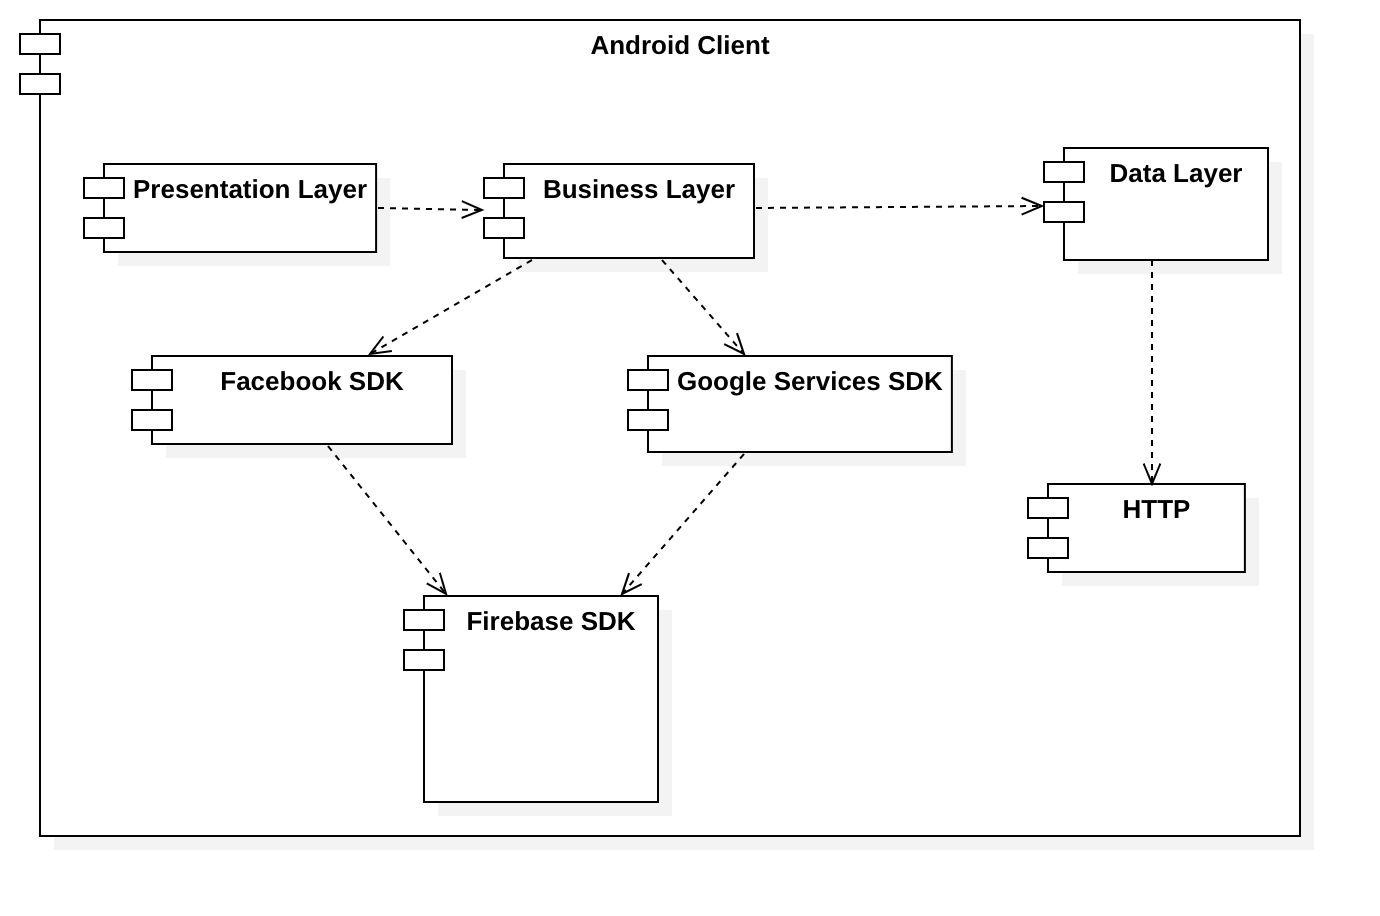
\includegraphics[scale=0.3]{androiddiagram}
  \caption{Android Component Diagram}
  \label{fig:android-component}
\end{figure}


\begin{figure}[H]
	\centering
  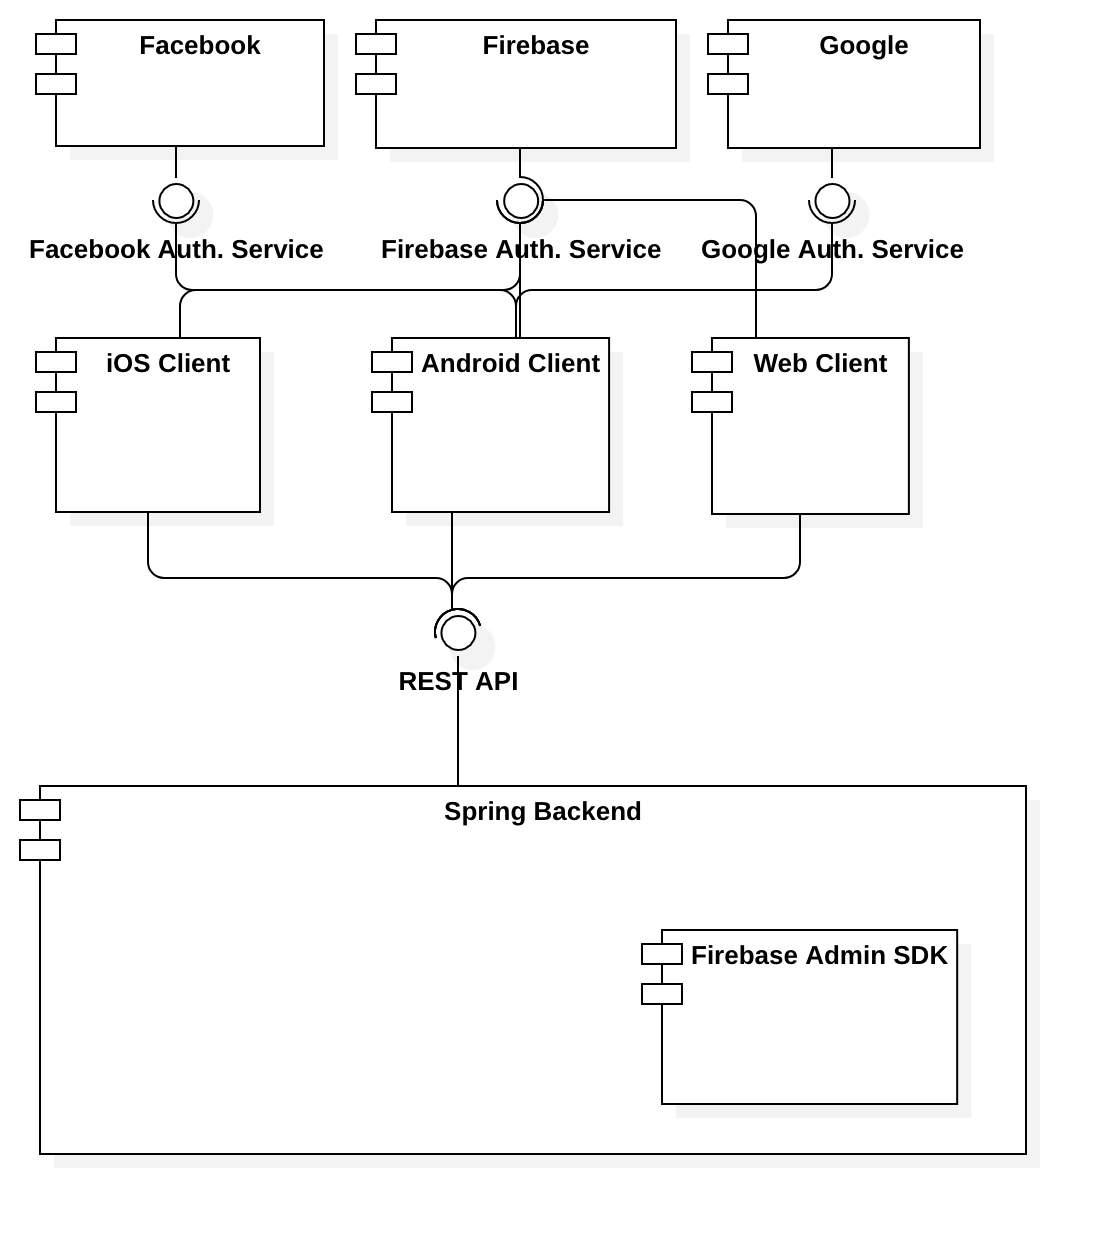
\includegraphics[scale=0.3]{systemdiagram}
  \caption{System Component Diagram}
  \label{fig:component}
\end{figure}



\newpage
\section{Domain Description}
 The Class Diagram in Figure \ref{fig:domain} represents the Domain Model of the application, it provides visual representation of Entities and relations between them. The design is based on the entities used on server-side.

\begin{figure}[H]
  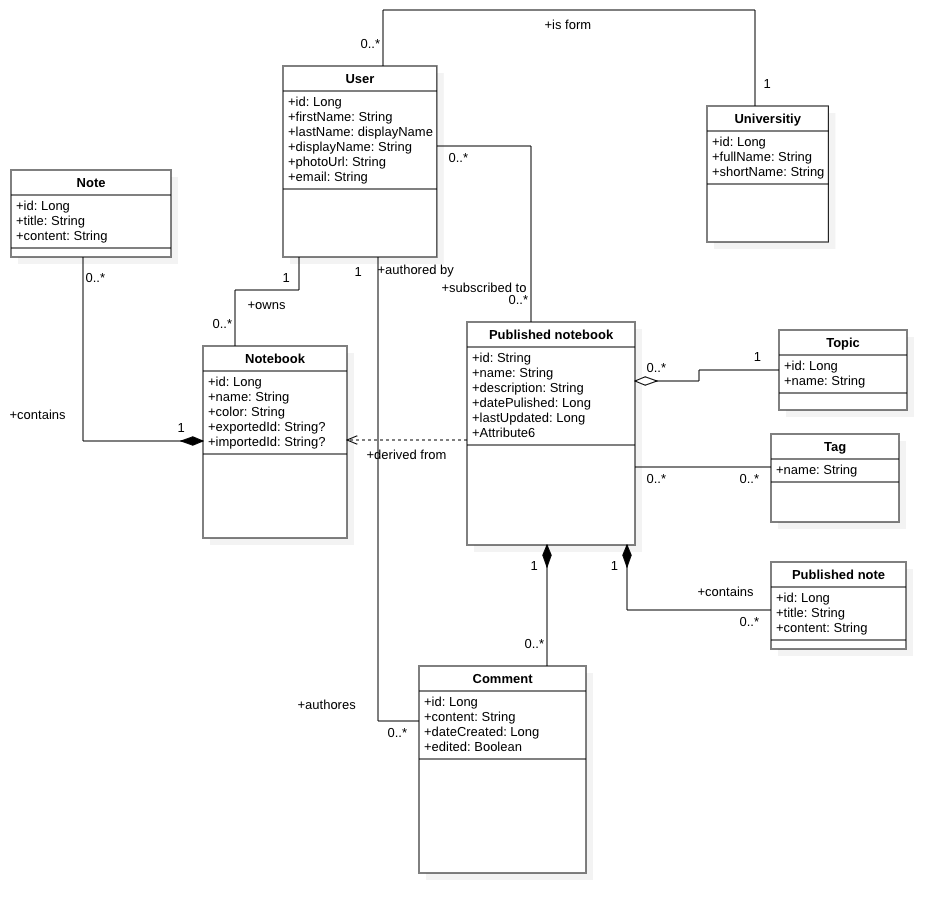
\includegraphics[width=\linewidth]{Domain}
  \caption{Domain Diagram}
  \label{fig:domain}
\end{figure}

 

\subsection{User}
	The User entity represents someone who has completed registration flow using one of the client applications or created manually (in case of Admin role). This entity contains such properties as: first name, last name, display name (automatically set as a combination of first and last names and photoUrl1. Due to the fact, that \appname\ provides several ways for the user to authorise, some of the properties will either come from the user's input or from the 3rd party API (such as Firebase).
	
\subsection{Note}
	Note represents a single piece of information. It consists of two properties: title and content. These can be described as term and definition or question and answer. Each note must be assigned to one of the notebooks, hence there is a 1:N relation.
\subsection{Notebook}
	Notebook is one of the main entities used in the application flow, and  can be created by an authenticated user. The soul purpose of the Notebook is to store Notes and serve as a source for a Published Notebook. Properties name and colour are used to help users distinguish between different Notebooks.
	
	
\subsection{University}
University represents a school, where the User can assign himself as a student during registration flow. It is used to unite users from the same school to make content searching easier. 

\subsection{Published Notebook}
Published Notebook represents a shareable content. It can be created by user, based on one of his/her notebooks by providing some additional details:
name, optional description,  topic and optional list of tags. All these properties are later used in a searching flow to optimise results.

\subsection{Topic}
Topic represents the main category or subject of the Published Notebook. Topic contains only one property -- its name.
\subsection{Tag}
Tag is a short label attached to the Published Notebook. It is mainly  used to narrow the topic or school. Tag has only one property -- its actual value stored as the name.

\subsection{Comment}
Users can comment on published notebooks. Most of the properties are assigned automatically, with the only exception being content: it represents the body of the comment and assigned by the user.

\subsection{Version State and Modification}
Version state and Modification are used to enable notebooks versioning system which in order to support Suggestions Requirements. Every Notebook, either local or published got its own Version state. Version state contains an identifier, version number, which is used for version comparison and list of the modifications that were done on top of the current version.


Modifications are like commits; it is a single notebook modification which is limited to a note update and a creation of a new one.  Modification contains several properties: an identifier, the id of the note that has been modified (if any) and the actual change stored as strings.

\newpage

\chapter{Design}
This chapter provides an insight into how \appname\ will comply with the requirements established previously.

\section{Material Design}
Material Design is a design language that Google developed in 2014. Later in 2018, it was revamped with a goal to provide more flexibility for designers to create more custom themes. Material Design was chosen as a main source of inspiration when creating \appname\ UI due following  reasons:
\begin{itemize}
	\item Material Design has very wide support on Android Platform. Every component that is described in Material Design Guidelines is implemented by Google and can be used by developers.
	\item Material Design is cross-platform, meaning that its guidelines can easily be applied when creating design for other platforms like iOS or Web.
\end{itemize}

\subsection{Used Components}
This section contains a list of Material Design specific Components (not including widely used elements such as Buttons and Input Fields) used when creating design for \appname.


\begin{itemize}
	\item \textbf{Floating Action Button (FAB)}: According to Material Design Guidelines: \quoting{A floating action button (FAB) performs the primary, or most common, action on a screen. It appears in front of all screen content, typically as a circular shape with an icon in its center}\cite{material-fab}. FAB is widely used in creating content, hence it found its place in the note-taking part of the application.
		\item \textbf{Chips}: \quoting{Chips are compact elements that represent an input, attribute, or action}\cite{material-chips}. In \appname\ it is used mainly for displaying Tags and in Searching flow. In most of the cases it will be placed inside the ChipGroup -- a special container to store dynamic amount of Chips
	\item \textbf{Bottom Sheets}: \quoting{Bottom sheets are surfaces containing supplementary content that are anchored to the bottom of the screen.}. The most common Bottom Sheet type used in \appname\ is Modal Bottom Sheet, that allows user to provide certain kind of input, like Topic, Tag selection and e.t.c.
	\end{itemize}

\section{UI \& UX}

This section contains most important screens description from UI \& UX standpoint, wireframes and its iterations.

\subsection{Library Management}
Library management requirements (F8-F15) are covered by the first top-level destination: \textbf{My Library}. This part of the application serves as the main entry point for the returning users. Wireframes of this sections can be viewed in Figure \ref{fig:section-library}.
	
	Its first screen, as shown in Figure \ref{fig:notebooks}, contains a scrollable list of Notebooks and provides access to the various notebook-management related actions such as: Notebook creation(triggered by FAB), edition, deletion and sharing (triggered by options menu button).
		
	By clicking on one of the notebooks in the list, user will be transferred to the Notes List Screen (Figure \ref{fig:notes}). Similar to Notebooks List Screen, this screen contains a scrollable list of notes from this notebook and  covers all the note management related actions and interactions such as Note creation, edition and deletion. Once again, FAB is used for to trigger a create action.
	
	Finally, by choosing a note, the user will be able to view its details. As shown of Figure \ref{fig:detail}, this screen utilises top app bar to provide access for the delete action. FAB is used to trigger the edit action.
	
\begin{figure}
\centering
\begin{subfigure}{.5\textwidth}
  \centering
  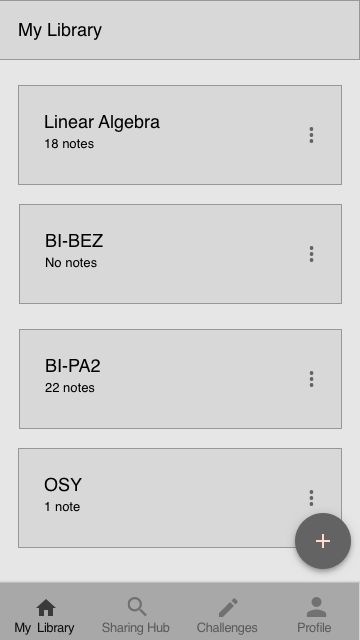
\includegraphics[scale=0.4]{Notebooks.png}
  \caption{Notebooks List Screen}
  \label{fig:notebooks}
\end{subfigure}%
\begin{subfigure}{.5\textwidth}
  \centering
  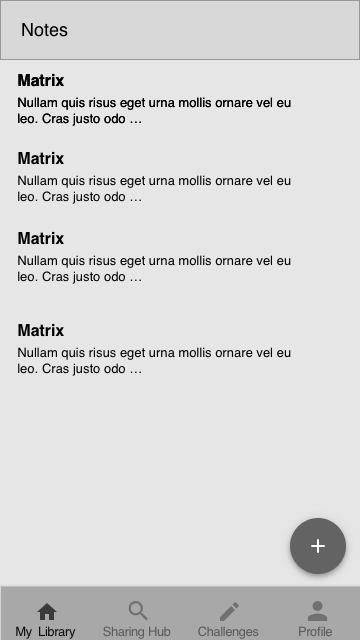
\includegraphics[scale=0.4]{Notes}
  \caption{Notes List Screen}
  \label{fig:notes}
\end{subfigure}
\begin{subfigure}{.5\textwidth}
  \centering
  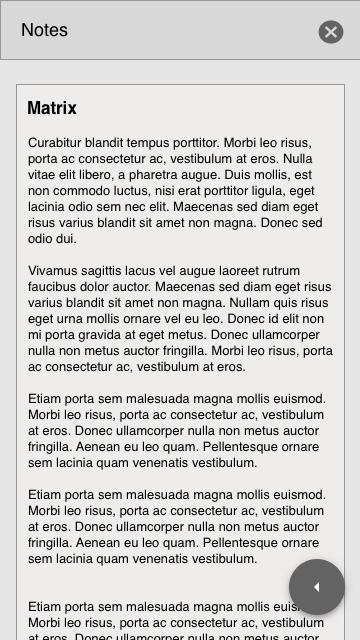
\includegraphics[scale=0.4]{NoteDetailView}
  \caption{Note Detail Screen}
  \label{fig:detail}
\end{subfigure}

\caption{My Library Section Wireframes}
\label{fig:section-library}
\end{figure}

\newpage
\subsection{Notebook Publishing}
The fact the all the content in \appname\ is made by its community makes Notebook Publishing Flow is one of the core functionalities of the application. The flow it self acts as complex form with different types of inputs:
\begin{itemize}
	\item Notebook name -- Single-line input field, will be pre-filled with the name of local Notebook that is being published.
	\item Language of the Notebook -- Selector, will be pre-filled with the current user locale.
	\item University/School associated with this Notebook -- Selector, will be pre-filled with the User's university, this field is optional.
	\item Topic/Category of the Notebook -- Selector, this field is mandatory.
	\item Tags -- ChipGroup, chosen tags will be represented by Chips. This field is optional.
	\item Description/Message for other users -- Multi-line input field, this field is optional.
\end{itemize}



Considering an amount of input needed, its variety, the decision was made to split this form into several steps. It will make the form more dynamic and put more emphasis on some inputs by grouping them.

First step will include all fields that can be pre-filled: Notebook's name, language and University. This will allow to skip first step in most cases, making it only about controlling pre-filled information.
Second step will require users to provide search-relevant information, such as Tags and Topic/Category, topic being a required option. Third step will allow user to provide a message or a more detailed of description of the Notebook. Fourth step will be all about confirmation, in which the user can double-check information he/she entered and submit it.

Though the choice of UI elements in different steps is well defined, they way we present these steps is not. Simplified wireframes with different approaches of how the steps can be presented are shown in Figure \ref{fig:publishing-sketches}. In the end, I made the decision to go with the Stepper solution as it gives a number of advantages:
	\begin{itemize}
		\item Stepper is a standardised element of Material Design.
		\item In every step, Stepper gives an overview of all steps available and its completion state.
		\item Stepper allows to quickly navigate between different steps.
	\end{itemize}
	
	More detailed wireframes for this flow using Stepper are shown of Figure \ref{fig:publishing-wireframe}.

\begin{figure}
\begin{subfigure}{.5\textwidth}
  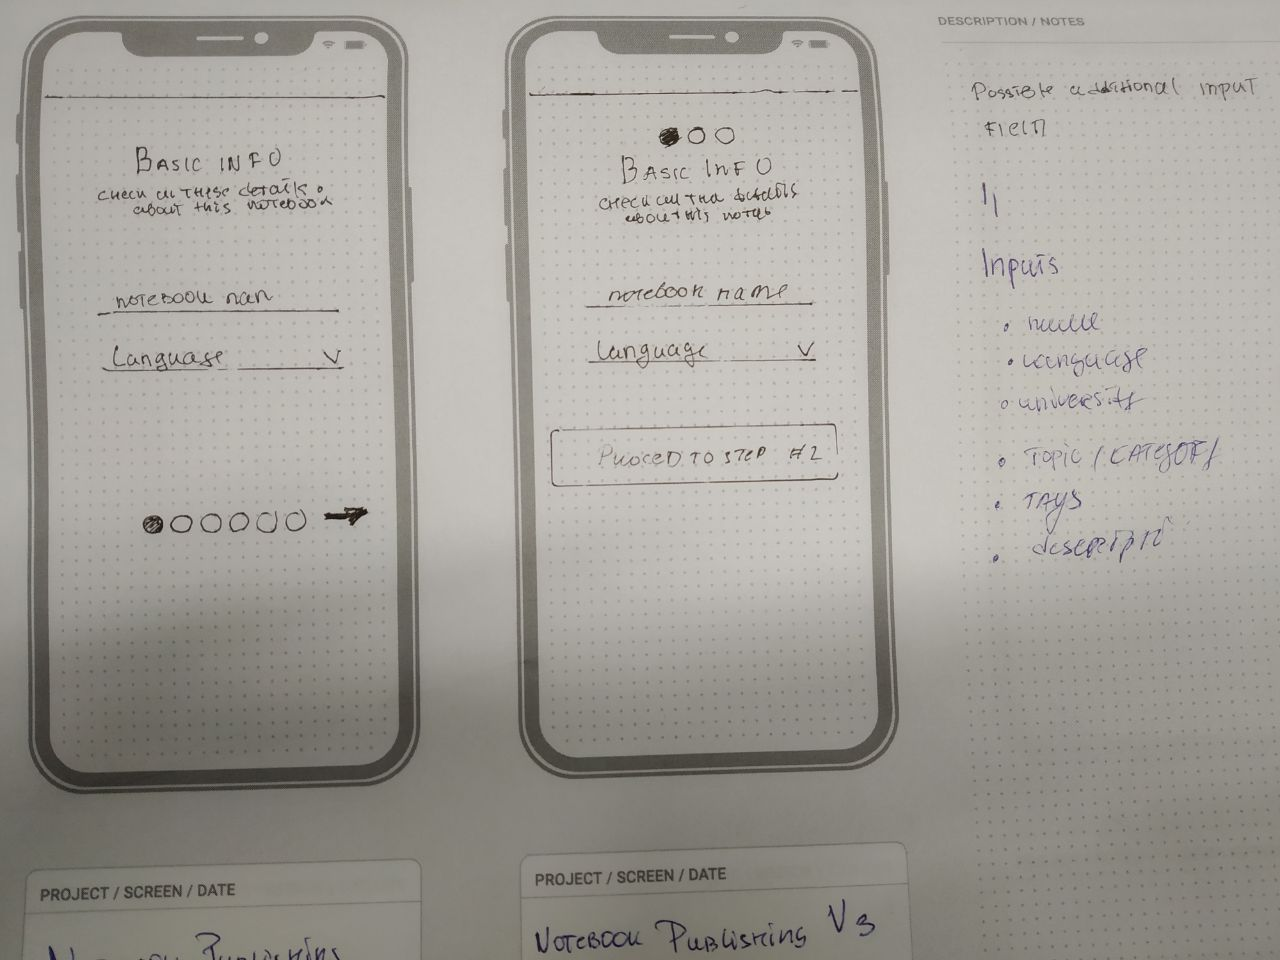
\includegraphics[scale=0.3]{publishing-sketches}
\end{subfigure}%

\begin{subfigure}{.5\textwidth}
  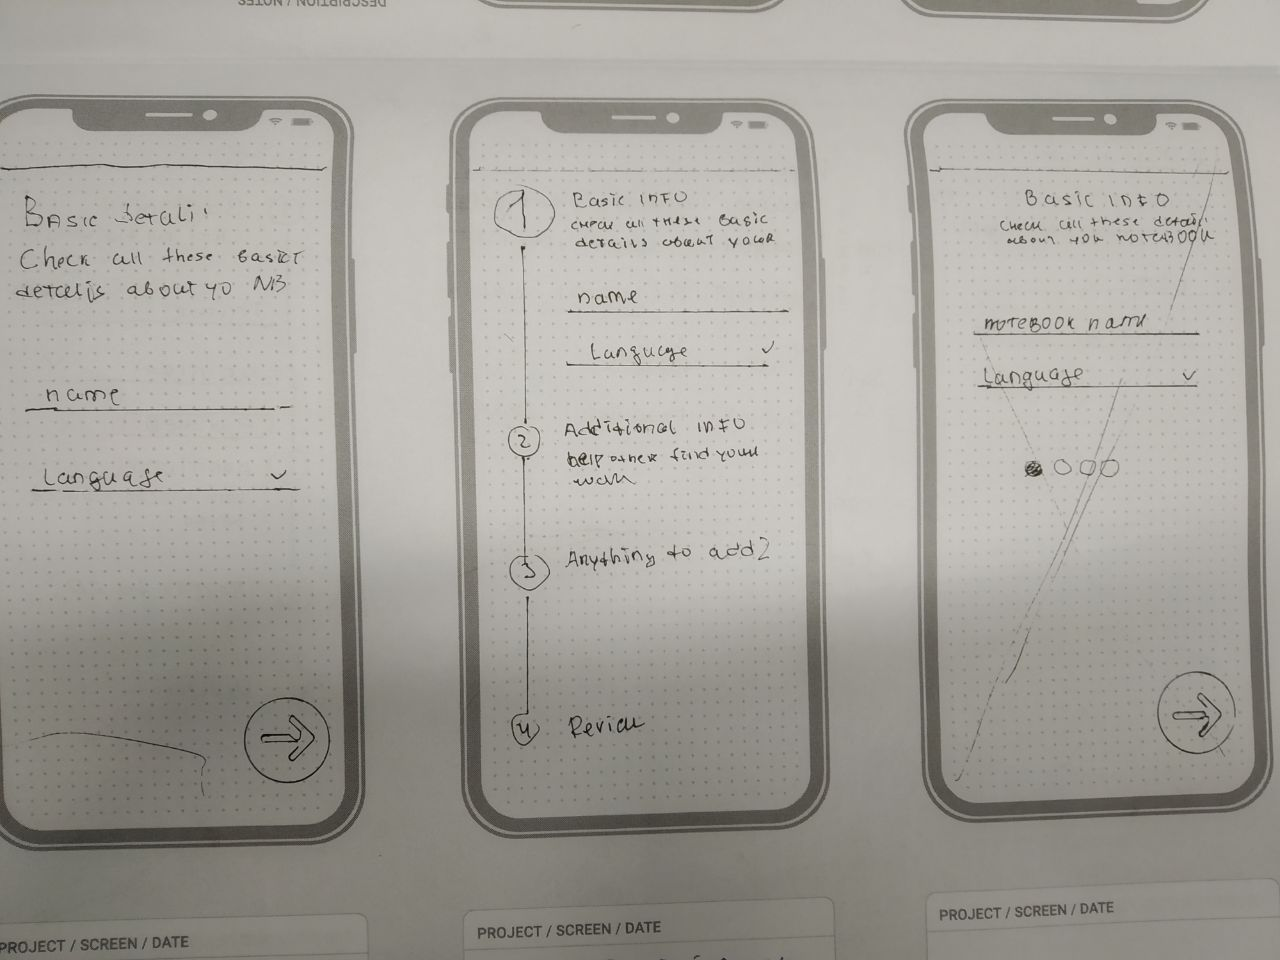
\includegraphics[scale=0.3]{publishing-sketches2}
\end{subfigure}

\caption{Notebook Publishing Flow - Sketch Phase}
\label{fig:publishing-sketches}
\end{figure}


\begin{figure}
\centering
\begin{subfigure}{.5\textwidth}
  \centering
  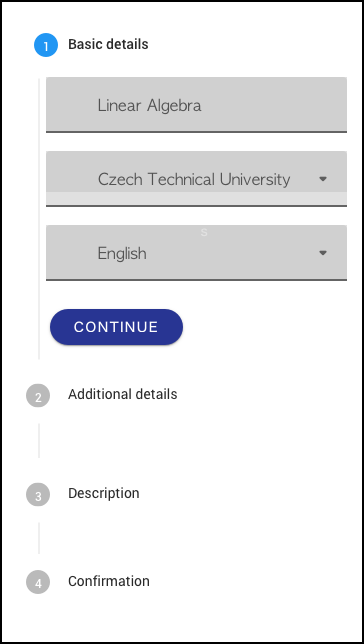
\includegraphics[scale=0.4]{step1}
  \caption{First Step of Notebook Publishing}
  \label{fig:step1}
\end{subfigure}%
\begin{subfigure}{.5\textwidth}
  \centering
  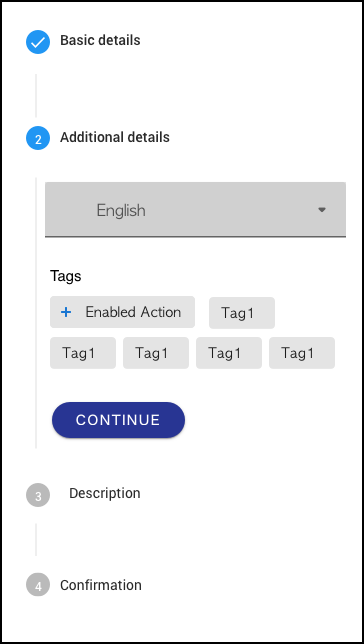
\includegraphics[scale=0.4]{step2}
  \caption{Second Step of Notebook Publishing }
  \label{fig:step2}
\end{subfigure}
\begin{subfigure}{.5\textwidth}
  \centering
  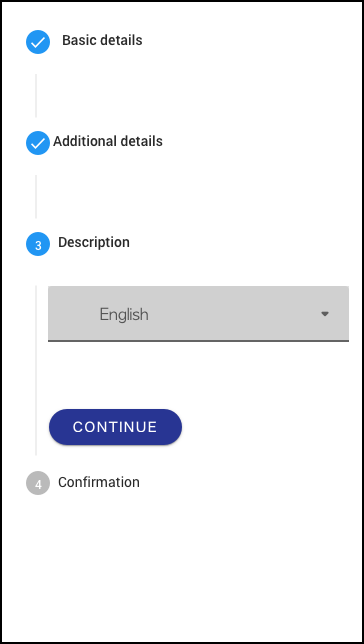
\includegraphics[scale=0.4]{step3}
  \caption{Third Step of Notebook Publishing }
  \label{fig:step3}
\end{subfigure}

\caption{Notebook Publishing Wireframes}
\label{fig:publishing-wireframe}
\end{figure}




\subsection{Sharing Hub}

\textbf{Sharing Hub} is another top-level destination, that allows users to access various Notebooks published by other users.

In the early stage of the \appname\ development, Sharing Hub root screen (Figure \ref{fig:section-sharinghubv1}) contained only one list with the Published Notebooks, with the idea of showing the most recently added Notebooks. Later on, the decision was made to make this screen more personalised by introducing Sections and Notifications preview (Figure \ref{fig:section-sharinghubv2sletch}).


Section is a small list of Published Notebooks of fixed size, that can be scrolled horizontally. By introducing these small lists it will be possible to group Published Notebooks into personalised sets (Notebooks from the user's university for example). Each Section is result of an executed query, so it can be used to facilitate the search flow. So, clicking the See All Button, will launch Search Flow with pre-filled search options, associated with this section.

Another newly added element is a Notifications preview. Located on the top part of the screen, this element displays notifications about the two most recent activities like Notebooks updates. By clicking the notification user will be to view the Notebook details associated with this notification.


\begin{figure}[!htbp]
\centering
\begin{subfigure}{.5\textwidth}
  \centering
 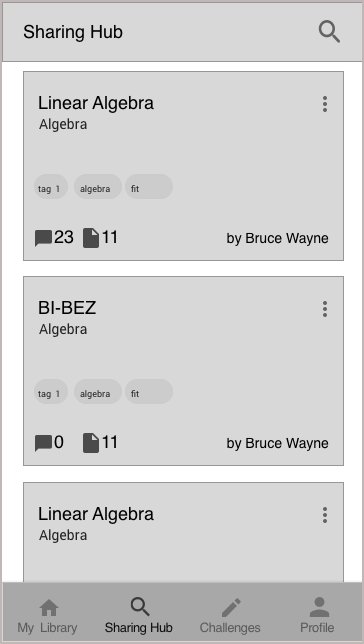
\includegraphics[scale=0.4]{SharingHub}
  \caption{Landing page v1}
  \label{fig:section-sharinghubv1}
\end{subfigure}%
\begin{subfigure}{.5\textwidth}
  \centering
  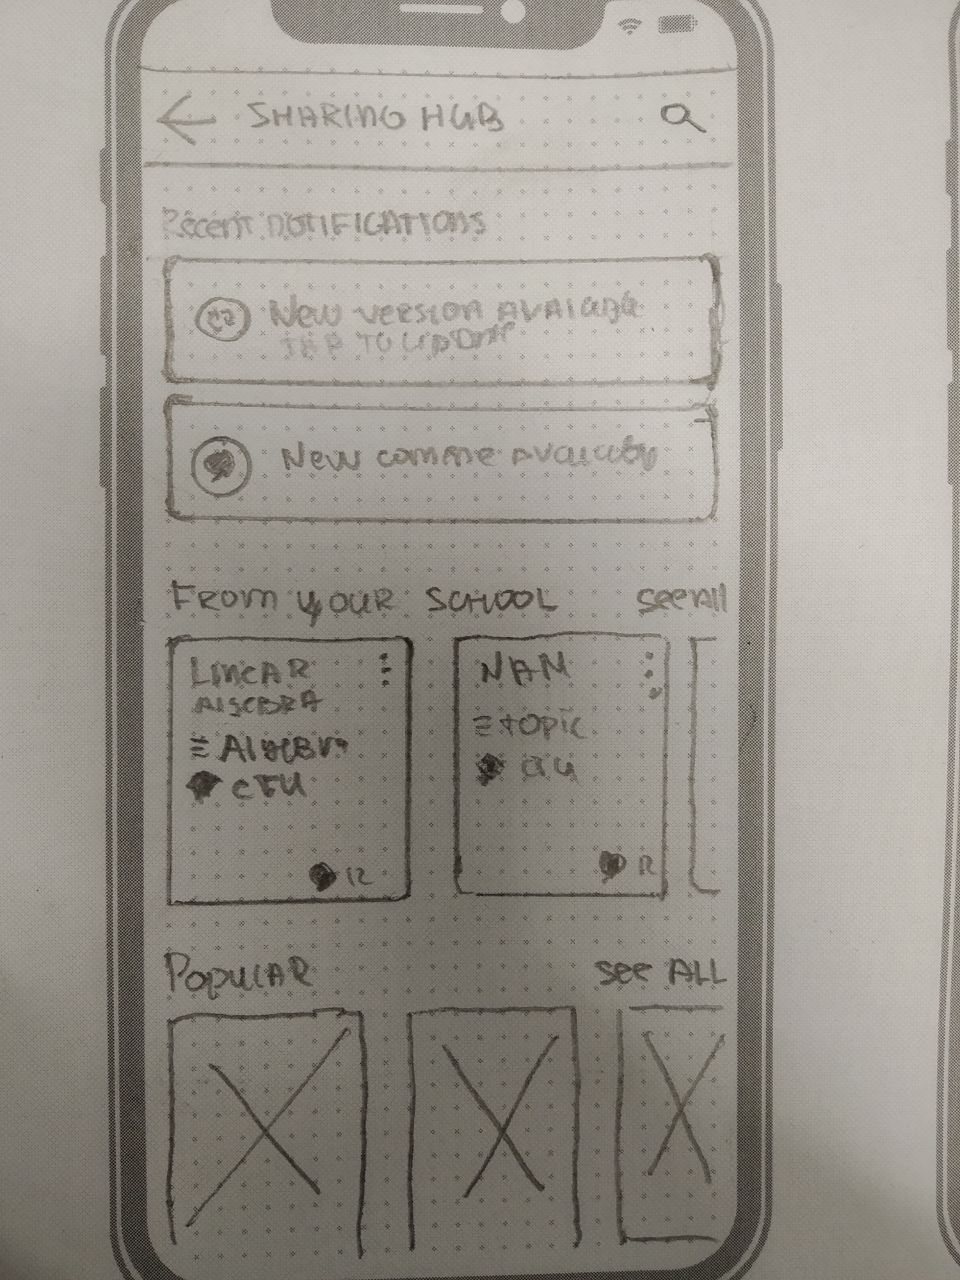
\includegraphics[scale=0.054]{sharingHubV2.jpg}
  \caption{Landing Page v2}
  \label{fig:section-sharinghubv2sletch}
\end{subfigure}

\caption{Sharing Hub Wireframes}
\label{fig:publishing-wireframe}
\end{figure}


\newpage
\subsection{Searching Flow}
 One of the main responsibilities of SharingHub screen is to start the Search flow. Search flow is either launched by a Search Menu Item located in the Top bar or by the expanding on expanding on the Notebooks Section. Here a list of some basic requirements that were taken into consideration:
 
 \begin{itemize}
 
 \item There are should several primary searching/filtering options available: Notebooks name, University/School, Topic/Category and Tags.
 \item All these options must be easily accessible with the idea that more searching options might be introduced during later phases of development.
 \item When none of searching options are active, empty state must be presented.
  \end{itemize}

The resulting wireframe is shown in Figure \ref{fig:section-search}. This approach is using a Top App bar to display active searching options. Each option is represented by a Chip action, that can have two states: Chip is either inactive  and displays the name of the search option, or it is active, displaying selected option's values. When there are a lot of values selected, in case of multiple Tags for example, last three selected will be shown. 

Clicking the Chip will result in showing Modal Bottom Sheet that will allow user to tweak selection of the active values and every change to a Search options values will result in updating the search results. Search results themselves appear in the scrollable list bellow the Top Bar. 
   

\begin{figure}[!htbp]
\centering
  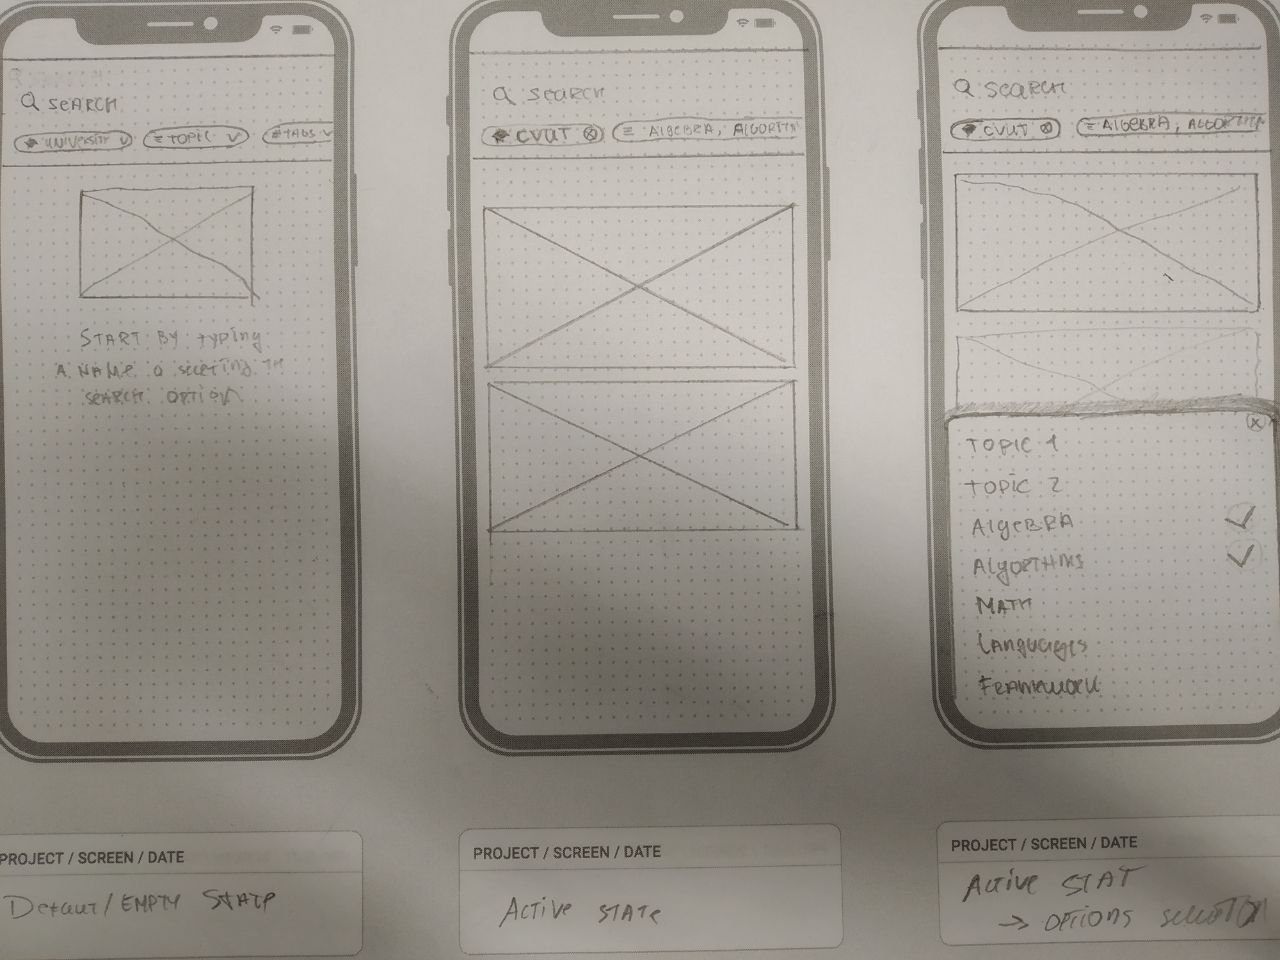
\includegraphics[scale=0.08]{sectionSearch}
  \caption{Search Flow Wireframes}
  \label{fig:section-search}
\end{figure}
 
\subsection{Published Notebook Details}
Published Notebook, as an entity, contains a large amount properties and there are a lot of actions associated with it. This screen will cover all actions regarding user comments (requirements F19-F22) and various Published Notebook actions such as saving, sharing, and copying. Including all these actions and flows into one screen would make UI very crowded, resulting in bad UX. \textit{Tabs} can help solve this issue quite easy.

According to Material Design Guidelines, Tabs can organise content across different screens, data sets, and allow navigation between groups of content that are related and at the same level of hierarchy\cite{material-tabs}. By using Tabs, this screen can be split into two distinct sections: Detail Tab and Comments Tab, thus dividing responsibilities and making this screen more user-friendly.
 

Details Tab (Figure \ref{fig:published-details}) features key details about this Notebook. Due to the fact that there are a lot of details to display, all the properties are  divided into several groups:


\begin{itemize}
	\item \textbf{Basic details}: This group contains simple properties such as Notebook's name, its author, category/topic, language and associated university.
	\item  \textbf{Description}: This group contains more dynamic content such as description, that can take multiple lines, and a Chip Group with tags.
	\item \textbf{Primary Notebook Action:} This view represents a primary action available for this notebook in regards to user Library. This can either act as a Save button, that will save the latest Notebook version to the user's Library or as an Update Button, that will result in applying changes from local notebook to the Published one, thus updating its contents. If none of the actions are available, this view will be hidden.
	 \item \textbf{Suggestions}: This view group serves as preview and an entry point for the suggestions screen. 
	\item \textbf{Notes Preview}: Last view at the bottom of the screen serves as an entry point for notes browsing.
\end{itemize}
 
Comments tab, as shown in Figure \ref{fig:published-comments}, contains a scrollable list of the user comments and an Input Field, that will be used to create a new comment, or edit the old one. Also, every comment contains an options button that can be used to trigger either an edit or a delete action.

\begin{figure}[H]
\begin{subfigure}{.5\textwidth}
  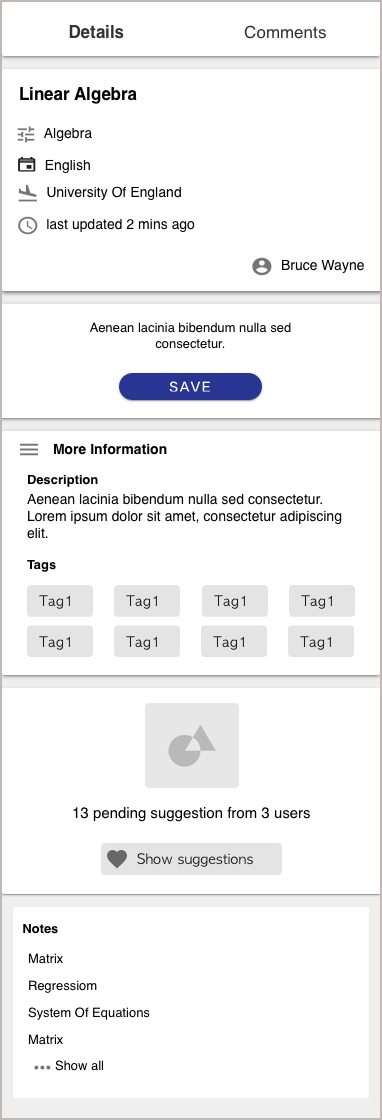
\includegraphics[scale=0.45]{comments}
  \caption{Details Tab}
  \label{fig:published-details}
\end{subfigure}%
\begin{subfigure}{.5\textwidth}
  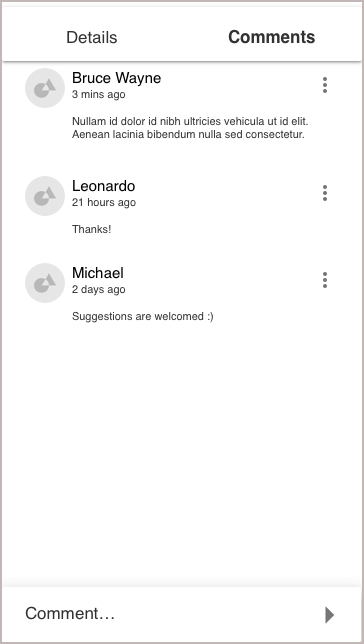
\includegraphics[scale=0.5]{details}
  \caption{Comments Tab}
  \label{fig:published-comments}
\end{subfigure}
\caption{Published Notebook Details Wireframes}
\label{fig:section-published}
\end{figure}

\subsection{Suggestions Review Flow}
As mentioned before, one of the actions provided by Published Notebook Detail Screen is to show a list of the suggestions left by other users.  Wireframe of this screen can be seen in Figure \ref{fig:suggestion-preview1}.  Besides the screen itself, there is also a FAB that will start the review flow; hence his button will be visible only to the Author of the Published Notebook.

\subsubsection{Review Process}
The wireframe of the review screen is presented in Figure \ref{fig:suggestion-review2}. There are three core parts to this screen. First, there is a list of the suggestions: they appear one by one, as a part of horizontal list, covering most of the screen's space. In case it is a new note it will only show one note card, in case it is an updated note, two cards will be shown: one with notes current data and one with the data suggested by a user. User is able to navigate inside this list using horizontal swipe gesture. Buttons below the suggestion will either mark the suggestion as approved or rejected, thus updating the second part: Review Status Bottom Sheet. 

\subsubsection{Review Confirmation}
Review status bottom sheet reflects the current status of the review process displaying how many suggestions are examined (approved or rejected). Expanding the bottom sheet (Figure \ref{fig:suggestion-review3})  will reveal an overview allowing the user to double check his/her input. This overview contains the same list as in Figure \ref{fig:suggestion-preview1} with the only difference being that it reflects the suggestion status. Scrolling to the end of this list will reveal the button that is used to submit the review. User will be navigated back to the suggestions list after the review submission.

\flushbottom

\begin{figure}[!htbp]
\begin{subfigure}{.5\textwidth}
  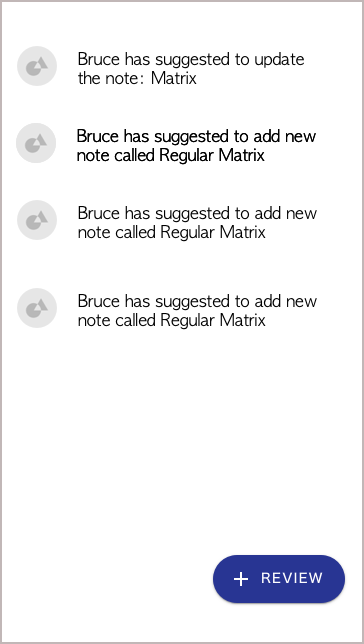
\includegraphics[scale=0.4]{review1}
  \caption{Pending Suggestions List Screen}
  \label{fig:suggestion-preview1}
\end{subfigure}
\begin{subfigure}{.5\textwidth}
  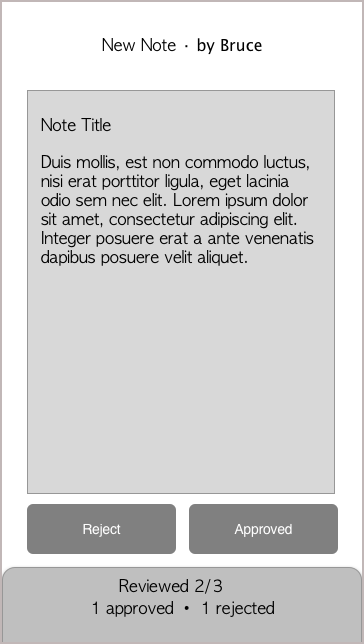
\includegraphics[scale=0.4]{review2}
  \caption{Suggestions Review Screen}
  \label{fig:suggestion-review2}
\end{subfigure}
\begin{subfigure}{1\textwidth}
\vspace*{5mm}
\centering
  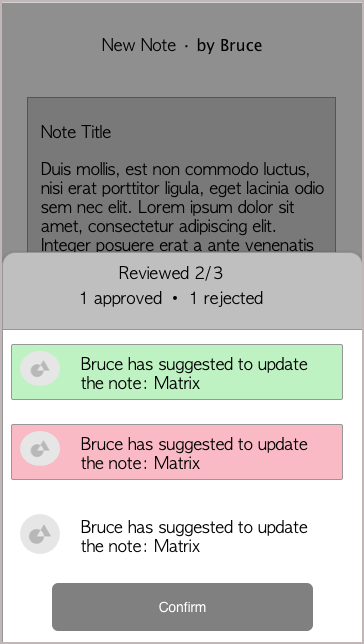
\includegraphics[scale=0.4]{review3.png}
  \caption{Suggestions Review Screen With Expanded Sheet}
  \label{fig:suggestion-review3}
\end{subfigure}

\caption{Suggestions Review Flow Wireframes}
\label{fig:section-published}
\end{figure}

\newpage
\subsection{Challenges}
The current iteration of \appname\ provides a small amount of very easy challenges (or tests) where user can test his/her knowledge of one of the notebooks. \textbf{Challenges} section serves as an entry point for setting up these different tests.


\subsubsection{Landing Screen}
Its landing screen (Figure \ref{fig:challenge-start}) features a list of recently completed challenges, including some statistics if available,  and three buttons, that are responsible for launching three distinct challenges: Flashcards, Write and Self-check. There is also a button that will navigate the user to a more in-depth configuration of his/her trial - Setup Challenge screen. Clicking one of the recently completed challenges entries will launch this challenge with all the options pre-set automatically. If the user hasn't completed any challenge yet, the empty view will be shown.



\subsubsection{Challenge Setup Screen}

Besides choosing the type of the challenge and the notebook, Setup Challenge screen (Figure \ref{fig:challenge-setup})  allows the user to select some additional options before generating his test such as order of the question and what will serve as an answer (either title of the note or its content). After all the details required are provided, most importantly challenge type and the notebook, the user will be able to start the test.

\subsubsection{Challenges Types}
Flashcard challenge is one of the simplest tests and requires no validation. Wireframe of this challenge can be seen in Figure \ref{fig:challenge-flash}.  This challenge is just an interactive way to walk through the notes, featuring a scrollable list of notes. User can flip the displayed flashcard to show the answer to a question and back. Navigation here doesn't have any restrictions so that the user can scroll it in any direction.  When reaching the end of the list, the user will see how many notes he/she studied.


Just like the Flashcards challenge, next test features a list of questions based on one of the users' notebooks. The idea of Self-check challenge (Figure \ref{fig:challenge-check}) is straightforward. Given a list of questions, the user must ask himself a simple question: do I know the answer? Two buttons below the flashcard are then self-explanatory: It's the user answer, either he/she know the answer or not. Clicking will "I know" will reveal the next question and clicking "Study again" will reveal the answer to the current question with the ability to go to the next one once the user is ready.

Write challenge (Figure \ref{fig:challenge})  is very similar to the Self-check challenge with the only distinction being that the user must provide his answer using an input field.
His answer will then be validated, and, depending on how close user was to the correct answer, it will either show next question or will require the user to re-submit his answer, correcting his/her mistake.

\begin{figure}[!h]
\caption{Challenges Screens Wireframes}
\begin{subfigure}{.5\textwidth}
  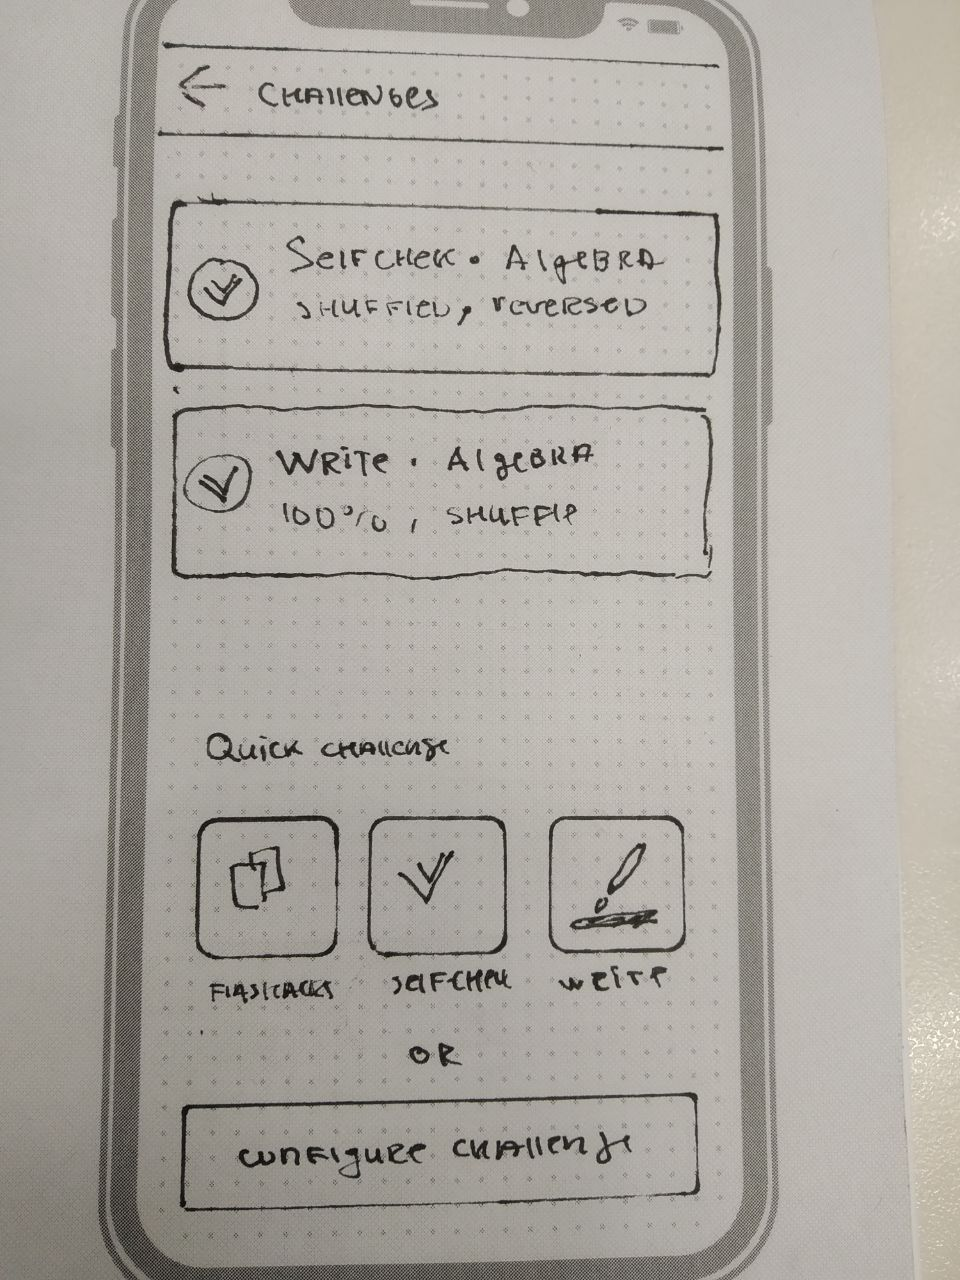
\includegraphics[scale=0.2]{challengesStart}
  \caption{Challenges Landing Screen Wireframe}
  \label{fig:challenge-start}
\end{subfigure}%
\begin{subfigure}{.5\textwidth}
  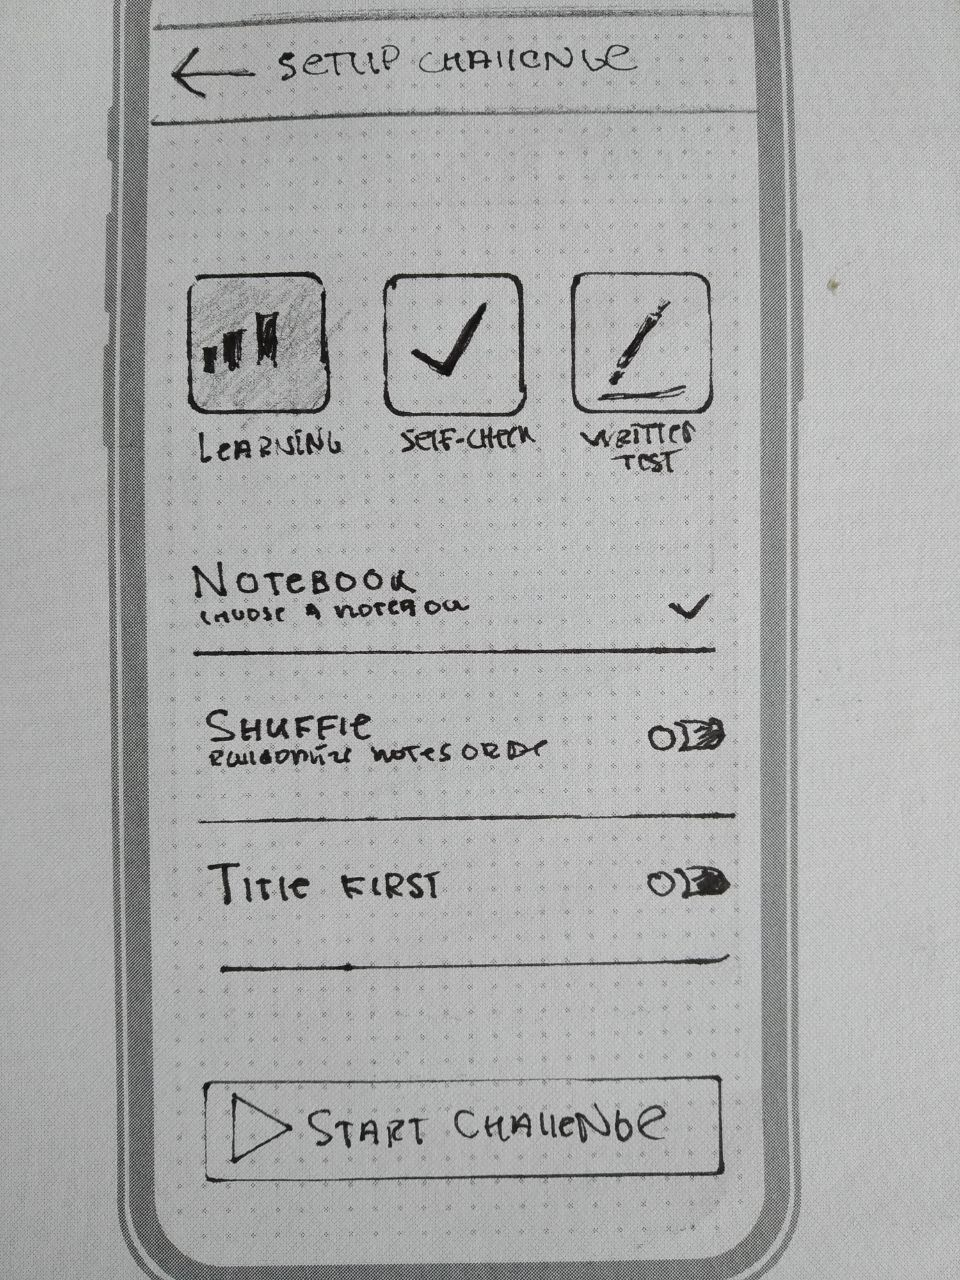
\includegraphics[scale=0.2]{challengesSetup}
  \caption{Setup Challenge Wireframe}
  \label{fig:challenge-setup}
\end{subfigure}
\end{figure}

\newpage

\begin{figure}[H]
\centering
\begin{subfigure}{.5\textwidth}
  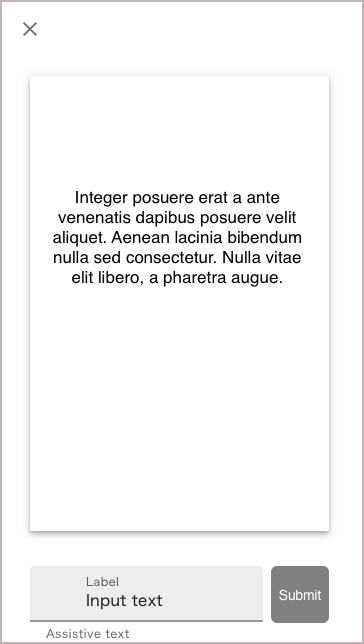
\includegraphics[scale=0.45]{write}
  \caption{Write Challenge Wireframe}
  \label{fig:challenge}
\end{subfigure}%
\begin{subfigure}{.5\textwidth}
  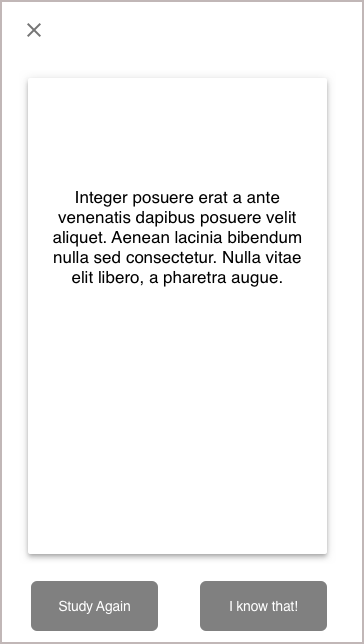
\includegraphics[scale=0.45]{selfcheck}
  \caption{Self-check Challenge Wireframe}
  \label{fig:challenge-check}
\end{subfigure}
\begin{subfigure}{.5\textwidth}
  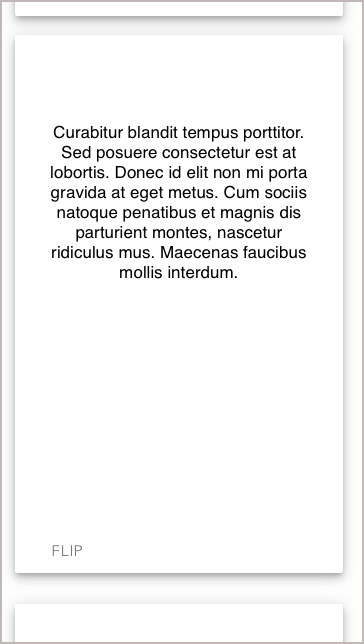
\includegraphics[scale=0.45]{flashcards}
  \caption{Flashcards Challenge Wireframe}
  \label{fig:challenge-flash}
\end{subfigure}
\end{figure}


\subsection{Profile}

\textbf{Profile} is the last top-level destination available from the Navigation bar. As shown in Figure \ref{fig:section-profile}, it features basic information about a currently logged-in user and provides buttons to access three more subsections: Profile Edition, Notifications, and Settings.

Profile edition screen (Figure \ref{fig:section-editprofile}) allows user to change his/her name and university. The screen contains two input fields that will be automatically populated with user information, and a Save button, that will only be enabled if one of the input fields changes. Pressing the Save button will try to update the information and navigate back to profile screen in case of success.

Notifications screen contains a scrollable list of all previously received notifications. It is the same component used in the Sharing Hub screen. Settings screen contains application-relevant information and preferences. One of the key functionalities there is a Logout button (requirement F34).


\begin{figure}[H]
\caption{Profile Screens Wireframes}
\begin{subfigure}{.5\textwidth}
  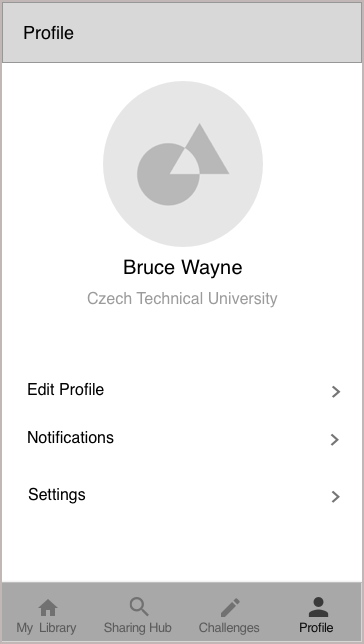
\includegraphics[scale=0.45]{profile}
  \caption{Profile Screen Wireframe}
  \label{fig:section-profile}
\end{subfigure}%
\begin{subfigure}{.5\textwidth}
  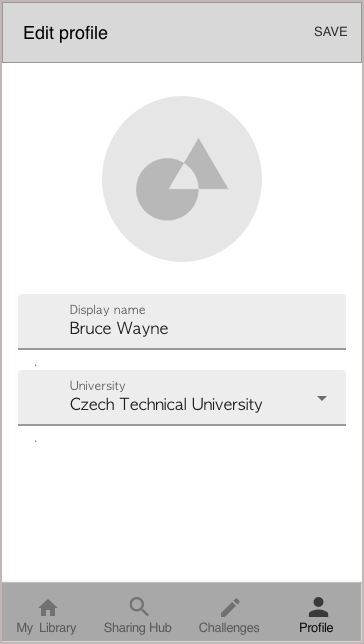
\includegraphics[scale=0.45]{editProfile}
  \caption{Edit Profile Screen Wireframe}
  \label{fig:section-editprofile}
\end{subfigure}
\end{figure}


\newpage 
\section{Application architecture}
On the of key requirements for \appname\ development is its architecture scalability. This section describes the approach chosen for its development and patterns in use.

\subsection{Android Architecture Components}
Previously, Google, as the leading Android contributor, never cared about the way developers build their applications. It has changed drastically with the introduction of Android Architecture Components (AAC) at Google I/O in 2017\cite{android-archguide}.
Architecture Components are a collection of libraries that can be used to design a robust and maintainable architecture.  LiveData and ViewModel components are the most important.  LiveData is a lifecycle-aware component is used to store data and notify its subscribers if the data changes.  ViewModel can store UI-related data and survive Activity Destruction which is especially useful in case of device rotation for example.

\subsection{Recommended Architecture}
Introduction of Architecture Components made it clear what approach Google recommends when designing application architecture -- MVVM. Figure \ref{fig-arch} demonstrates this approach:
\begin{itemize}
	\item Fragments and Activities represent the View.
	\item View is connected to a ViewModel. ViewModel there is represented by a ViewModel Architecture component that stores model data using LiveData, that Fragment or Activity can subscribe to. ViewModel requests data from the repository, without knowing where the data comes from.
	\item A Repository pattern represents the Model layer. Repository's responsibility is to retrieve and modify the data using one or multiple sources. Typically there is remote data source (API) and the local data source (in-memory database).
\end{itemize}

\begin{figure}
	\centering
  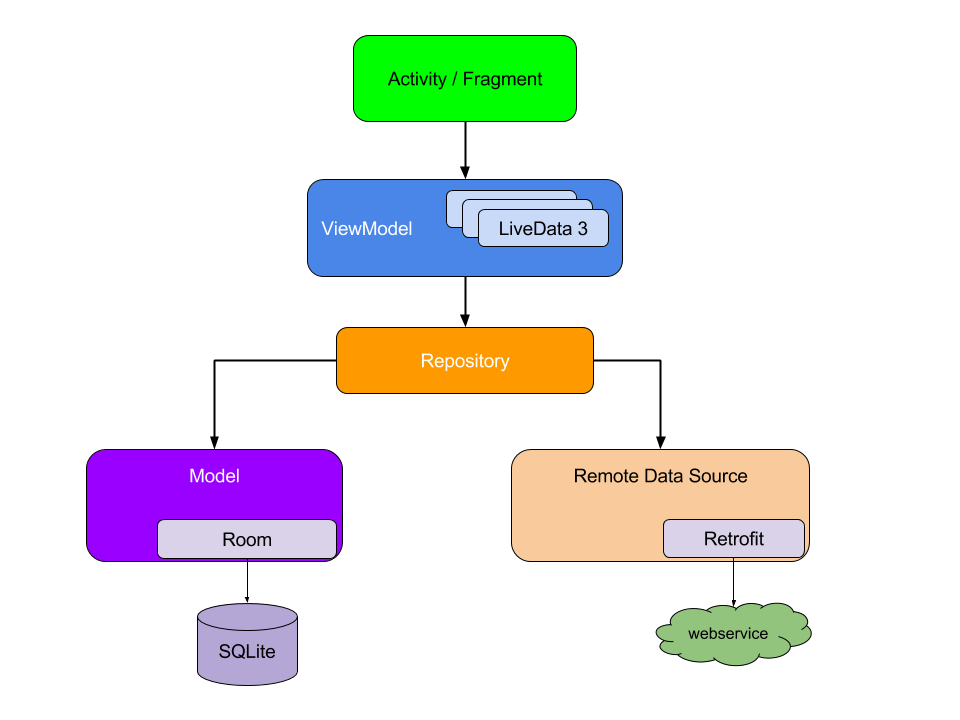
\includegraphics[scale=0.4]{final-architecture}
  \caption{Architecture Example Diagram\cite{android-archcomponents} }
  \label{fig-arch}
\end{figure}


\subsection{Chosen Architecture}
The fact that the MVVM  pattern is recommended by the developers of the Android OS and the existence of Architecture Components makes MVVM a solid choice and a good starting point for the application architecture. 


\appname\ will follow the recommended architecture with the exception of adding of one more clean architecture pattern -- Interactor (or use-case).


\subsection{Repository}
Repository is an abstraction that deals with the Entities. Repository can have one or multiple data sources. One of the main \appname\ data sources is its REST API. In-memory database will act as a secondary data source to allow some offline capabilities. 

\subsection{Interactors}
Though the repository pattern is a great abstraction for data layer, it would make sense to go even further and apply more Clean architecture principles. Interactor, or a Use-case, is another abstraction that represents a single use-case -- one rule of business logic. Interactor is usually talks to the repository and then returns the result to the caller.

This will even more propagate the separation of concerns as every Interactor will only deal with one particular functionality, which will make code more clear and make uni-testing easier in the future.


\subsection{Dependncy Injection}
 Dependency injection (DI) is basically providing the objects that an object needs (its dependencies) instead of having to construct them manually.
DI is another technique that will help provide cleaner code and will be a great help when providing a test-coverage. 

\subsection{\appname\ Architecture}
Overall architecture will include following components:
\begin{itemize}
	\item \textbf{Presentation Layer}, that is represented by \texttt{Fragments} and \texttt{Activities}. They are only aware about how to display information and does not contain any complex logic. All the interactions are getting handled by Domain Layer
	\item \textbf{Business Layer} is represented by \texttt{ViewModel}. ViewModel is injected into the Presentation Layer, it handles all user interactions and decides what and when to display, including navigation. ViewModel also executes Interactors and handles its result.
	\item \textbf{Data Layer} is represented by Interactors and Repositories. Interactors get injected into ViewModel and serves to execute certain request in the background and provide a result via callbacks. Repositories provide Entity-based operations using the data sources.
\end{itemize}
 
\chapter{Implementation}
This chapter describes main pin points of \appname\ implementation, platform-specific technologies and libraries. 


\section{Used Libraries and Technologies}

\subsection{DI Framework}
There are a few DI frameworks available for Android, \texttt{Dagger} being one of the most popular. Dagger is a fully static  Java DI framework that uses annotations for dependencies resolution. Dagger got huge support from the developers' community, mainly because of its performance. All dependencies are resolved and generated during the building phase, thus making the application perform faster. But,  Dagger is pretty old, complex and requires a lot of boilerplate code to function properly. Introduction of Kotlin paved a way for new libraries to compete with Dagger.

\texttt{Koin} is a lightweight dependency injection framework written in pure Kotlin. Koin uses DSL for modules declaration and, as opposed to Dagger, it is very easy to use. And one of its most significant advantages: It provides \texttt{ViewModel} support out of the box us by using just a ViewModel keyword. Listings \ref{code:dagger} and \ref{code:koin} shows the example of declaring and injecting \texttt{ViewModels} using Dagger and Koin respectively. This example shows quite well how easy it to use Koin comparing to Dagger.

Because of its great features, simplicity and the desire to make this application as modern as possible, Koin was chosen as the DI framework for \appname.
\newpage
\begin{lstlisting}[caption={ViewModel Injecting using Koin}, label={code:koin}, language=Kotlin]

// Define the dependency     
viewModel { LoginViewModel(get(), get(), get(), get()) }

// Inject into the fragment/activity
private val viewModel: LoginViewModel by viewModel()

\end{lstlisting}

\begin{lstlisting}[caption={ViewModel injecting using Dagger}, label={code:dagger}, language=Kotlin]
   
@Binds
@IntoMap
@ViewModelKey(MainActivityViewModel::class)
abstract fun bindViewModel(
viewModel:MainActivityViewModel): ViewModel

@ContributesAndroidInjector
internal abstract fun mainActivity(): MainActivity

// Inject factory
@Inject lateinit var factory: ViewModelProvider.Factory

// Build viewModel
private val viewModel = ViewModelProviders.of(
			this, viewModelFactory)
           		.get(VM::class.java)

\end{lstlisting}

\subsection{Retrofit}
Retrofit is a library that serves as a HTTP  client. Nowadays it is pretty much an industry standard, and it is hard to argue with it. Retrofit provides a type-safe way to describe your HTTP API using Java/Kotlin interface and annotations, transforming your API into just one interface.

 Annotations allow to modify the requests options and parameters such as request type, body or query parameters. For example, Listing \ref{code:retrofit} demonstrates a call to update a Notebook by id. \texttt{@PATCH} annotation serves to specify the type of the request to be performed, \texttt{@Path} represents the part of the requests path and \texttt{@Body} is a request body that will be converted into JSON.


Retrofit also has support for some popular threading libraries like RxJava, and recently -- Kotlin coroutines, allowing to specify the return type as \texttt{Deferred}.

\newpage
\begin{lstlisting}[caption={Retrofit Call Example}, label={code:retrofit}, language=Kotlin]


@PATCH("$API/notebooks/{id}")
    fun updateNotebookAsync(
    @Path("id") id: String,
    @Body body: Body) : Deferred<NotebooksResponse>

   
\end{lstlisting}


\subsection{Threading}
Threading and background work has always been a problem in the world of Android development.  Google provided some tools and APIs to solve this problem: AsyncTasks and Loaders. Both of them have a lot of issues, mainly because they are not very intuitive and not flexible to use. AsyncTask specifically, when not used properly, was the main cause for memory leaks.

Later on, RxJava gains popularity. RxJava is a library for composing asynchronous and event-based programs by using observable sequences. It is a very powerful tool, but the library itself is quite heavy (almost 2 MB), and when used only for threading it is often described as an attempt to kill a spider with the bazooka.

Kotlin has its own way to handle background work. Kotlin 1.3 introduced the Kotlin Coroutines.   Coroutines can be described as light-weight threads and essentially its a small task that normal thread can execute. Kotlin uses a concept of \texttt{suspending} functions, that is a regular function with the \texttt{suspend} modifier which indicates that the function can suspend the execution of a coroutine. This essentially allows to write asynchronous code that looks like synchronous making the code far more understandable and easy to read.
When it comes to \appname, Kotlin Coroutines are mainly used in the applications data layer: in Interactors and Repositories.

\subsection{Android Navigation Component}
Navigation in Android can be done either by using Activities or Fragment transactions. Android Architecture Components introduced a new way to solve navigation -- Navigation Component.

Navigation Component serves as an abstraction layer above \texttt{FragmentManager} that is used to manage fragment transactions. Navigation Component handles a lot of things:
\begin{itemize}
	\item Handles back stack management.
	\item Provides utility methods for commonly used UI Elements such as Toolbar, BottomNavigationBar, and e.t.c.
	\item  Provides a type-safe way to pass arguments between destinations.

\end{itemize}

Navigation is described using XML, Android  Studio also provides a visual editor for it to build your navigation graph (Figure \ref{fig:navigationeditor}). Navigation itself is handled by Navigation Controller, which resolves destinations available and does the Fragment transaction under the hood.

\begin{figure}
	\caption{Navigation Editor}
	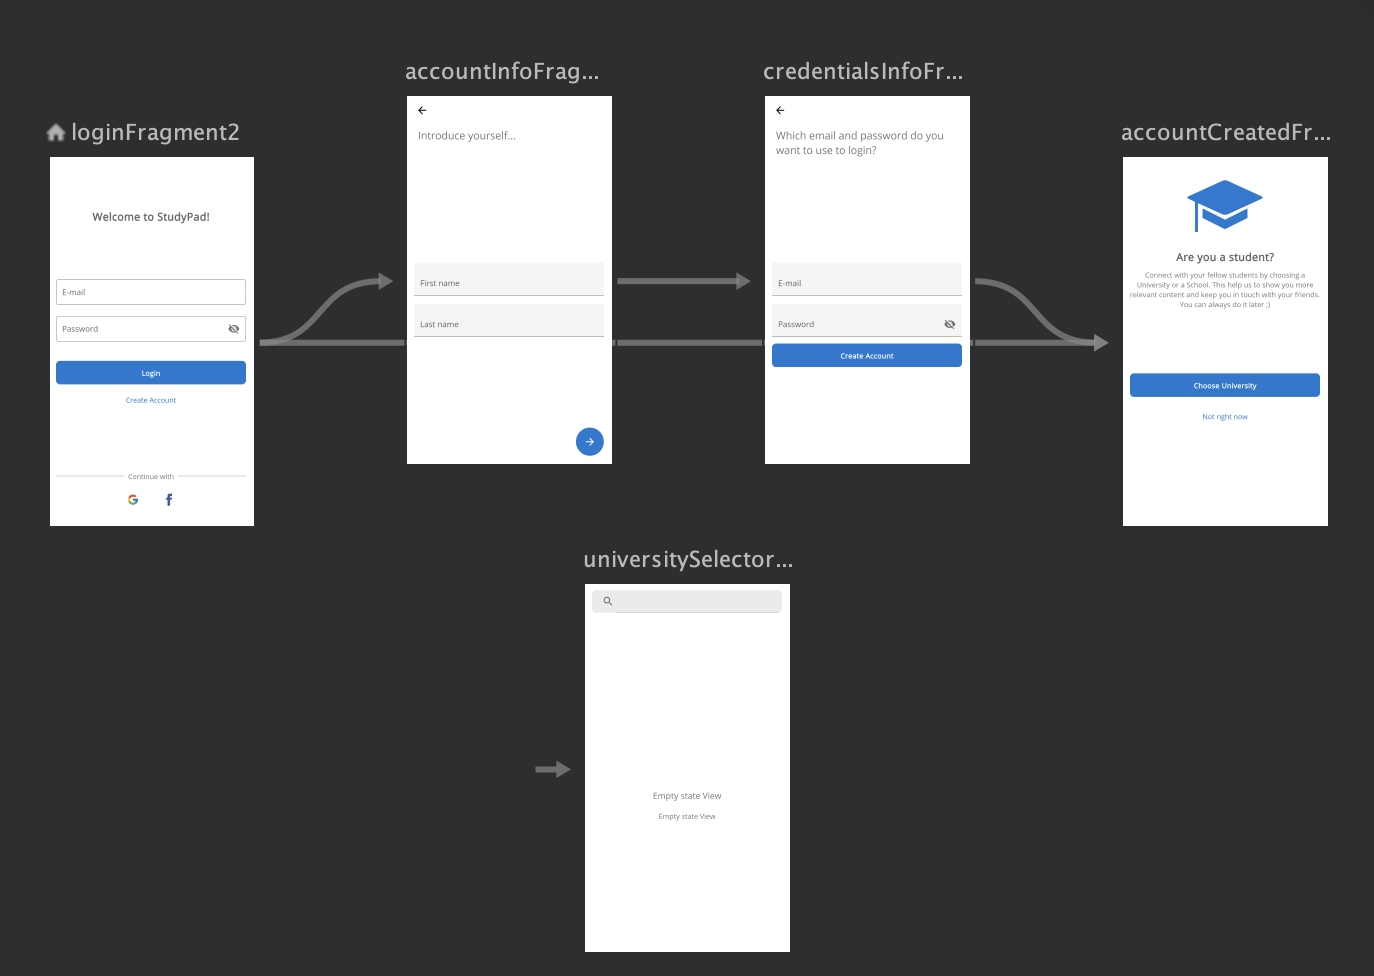
\includegraphics[width=350pt,height=300pt]{navigationeditor}
	\label{fig:navigationeditor}
\end{figure}

\subsection{ViewModel}
One of the essential parts of AAC is ViewModel. \texttt{ViewModel} is the implementation of the ViewModel pattern provided by Google as a part of AAC.
One of the key features of the ViewModel -- it can survive configuration changes. 

Activity's lifecycle is on the of most problematic concepts in Android Development: because every configuration change, such as phone rotation for example, destroys shown Activity and it must be recreated, thus causing a lot of issues due to the lost UI state. ViewModel lifecycle is different. As shown in Figure \ref{fig:1}, the ViewModel remains in memory until the Lifecycle it's scoped to goes away permanently: in the case of an activity, when it finishes, while in the case of a Fragment when it's detached. The fact that ViewModel can survive configuration changes make ViewModel a perfect view state holder.

\begin{figure}
	\centering
	\caption{ViewModel lifecycle\cite{viewmodel-lc}}
	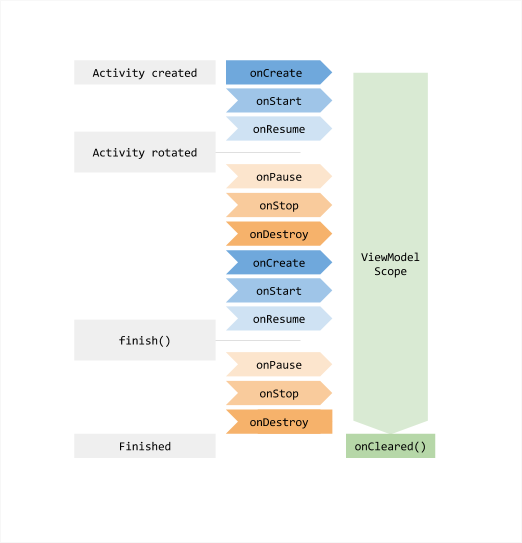
\includegraphics[scale=0.7]{viewmodellf}
	\label{fig:1}
\end{figure}

\subsection{LiveData}
LiveData is another useful tool from the AAC. LiveData is an observable, life-cycle aware data holder class, that goes hand-in-hand with ViewModel. Fragment or Activity can subscribe for updates and LiveData will notify its subscribers when new data is available, allowing them to update themselves accordingly. 
Because LiveData is lifecycle-aware it allows avoiding memory leaks and can easily be used to restore view state after the configuration change.


\section{Architecture Implementation}
There are four three important parts to the architecture implementation:
ViewModels, Interactors,  Repositories, and Activities with Fragments.
\subsection{Repository}
Repository acts as a single source of truth for the Interactors. Almost all of them are dependent on the remote data source --  API class provided by Retrofit, with the only exception  being Notebook repository, which also has a database dependency.

Listing \ref{code:repo} demonstrates implementation of the \texttt{getNotebooks()} method, which is marked as suspend. This allows using all the power of the Kotlin Coroutines. Retrofit got a Kotlin Coroutines support, allowing use of generic   \texttt{Defered} class as a return type, that is then used to wait for the result.

\begin{lstlisting}[caption={Repository Implementation Example}, label={code:repo}, language=Kotlin]
class NotebookRepositoryImpl(
    private val localDataSource: AppDatabase,
    private val remoteDataSource: Api
) : NotebookRepository {

/**
/* retrurns a list of the notebooks received from the api
/* and save the result into database
*/
override suspend fun getNotebooks(): List<Notebook> {
// wait for the api request to finish
  val list = remoteDataSource.getNotebooksAsync().await()
  localDataSource.notebookDao()
  	.putAll(list.map { it.toDomain() })
  return list
 }
 // other methods


\end{lstlisting}

\subsection{Interactors}
Interactors are used to perform one single use-case, or in other words, one single business logic operation. There are a lot of ways an interactor can be implemented. Sometimes it makes sense to make the interactor return LiveData, some times it is easier to handle the operation result via callbacks. Interactors in StudyPad mostly  relies on callbacks.

Every Interactor in \appname\ extends \texttt{BaseInteractor} or \newline \texttt{BaseInputInteractor} (when the opearation requires input). BaseInteractor, is an abstract class, it shortened implementation can be seen on Listing \ref{code:interactor}. This implementation fully relies on Kotlin Coroutines to execute the request in the background and provide a result using callback. 
This implementation of Interactors makes them very easy to declare, the only thing that has to be specified the actual action to be performed. The example of the resulting interactor can be seen on Listing \ref{code:logininteractor}.



\begin{lstlisting}[caption={BaseInteractor Implementaion}, label={code:interactor}, language=Kotlin]
abstract class BaseInteractor<T> {

  private var parentJob: Job = Job()
  var ioContext = Dispatchers.IO
  var mainContext = Dispatchers.Main

  protected abstract suspend fun runInBackground(): T

  fun execute(block: CompletionBlock<T>) {
    val response = Request<T>().apply { block() }
    unsubscribe()
    parentJob = Job()
    CoroutineScope(mainContext + parentJob).launch {
        try {
           val result = withContext(ioContext) {
                runInBackground()
             } catch(e: Exception) {
                 handleException(e)
               }
            }
        }
    }
 }
\end{lstlisting}

\newpage
\begin{lstlisting}[caption={LoginInteractor Example}, label={code:logininteractor}, language=Kotlin]
class LoginInteractor(private val repo: KeychainRepo) : 
BaseInputInteractor<LoginInteractor.Input, Unit>() {

 data class Input(val email: String, val password: String)

 override suspend fun runInBackground(input: Input) {
   val email = input.email
   val pwd = input.password
   return keychainRepository.login(email, pwd)
  }
}\end{lstlisting}

\subsection{Applying ViewModel and LiveData}
\texttt{ViewModel} in \appname\ manages three things:
\begin{itemize}
	\item Navigation,
	\item Interactors execution,
	\item And stores current view's state.
\end{itemize}

To make the development process a bit easier, I have created an abstract class \texttt{BaseViewModel} class for all the others ViewModels to extend. \texttt{BaseViewModel} contains two \texttt{MutableLiveData} instances. First one is  \newline \texttt{baseViewStateLiveData}. It holds a view state, that is the most common for every view: loading progress and error event. The second and the last one is \texttt{navigationEventLiveData}, that handles navigation events and commands.  This allows tot easily change view state using helper functions provided by BaseViewModel (Listing \ref{code:baseviewmodel}) in its subclasses. 



\begin{lstlisting}[caption={BaseViewModel methods}, label={code:baseviewmodel}, language=Kotlin]

protected fun toggleLoading(loading: Boolean) {
  val oldState = viewStateLiveData.value
  val updatedState = oldState.copy(isLoading = loading)
  viewStateLiveData.postValue(updatedState)
}

fun navigateBack() {
    val backEvent = NavigationEvent.NavigateBack
    navigationEventLiveData.call(backEvent)
}

protected fun navigateTo(direction: NavDirections) {
   val navEvent = NavigationEvent.NavigateTo(direction)
   navigationEventLiveData.call(navevnt)
}
 
 \end{lstlisting}

It is important to mention that the way \texttt{LiveData} manages its data is not perfect for some events. There are some events that should be triggered only once, like showing an error, confirmation message or navigating user to another screen. For this reason, I have created a \texttt{Event} class (Listing \ref{code:event}). \texttt{Event} is very simple generic class that holds a data and only allows to handle this data once. Event handling is done using \texttt{handle()} function, that accepts the lambda function, that will be invoked only once. All the error events and navigation events are using this class.

\begin{lstlisting}[caption={Event class}, label={code:event}, language=Kotlin]

class Event<out T>(private val content: T) {

    private var isAlreadyHandled: Boolean = false
    fun handle(block: (T) -> Unit) {
        if (!isAlreadyHandled) {
            isAlreadyHandled = true
            block.invoke(content)
        }
    }

}
 \end{lstlisting}
 
 
 Interactor execution usually results in updating the current screens View State, an example of this process can be seen on Listing \ref{code:viewmodelex}. This is just on of the many example that illustrates the flow of the data in the application.
 \begin{lstlisting}[caption={Usage of LiveData and Interactors in ViewModel}, label={code:viewmodelex}, language=Kotlin]

 // Update base view state to show loading
 toggleLoading(true)
 // Execute the interactor
 getRelevantNotebooks.execute {
    // Handle success 
     onComplete { result ->
        toggleLoading(false)
        // Transform notebooks to a displayable type
        val notebooks = result.map { it.toDomain() }
        // post new value
        liveData.postValue(notebooks)
      }
      onError {
        // handle error
        toggleLoading(false)
        handleApplicationError(it)
     }
 }
 \end{lstlisting}

\subsection{Present Data in Fragments}
The Activity in \appname\ serves only as a container for Fragments, thats why the actuals screens and flows are represented by Fragments. Just like with the \texttt{BaseViewModel}, I have created a basic definition of Fragment, that others fragments can extend -- \texttt{BaseFragment}.

\texttt{BaseFragment} provides a couple of helper methods that are used across the application and automatically subscribes for the two LiveData instances available from the \texttt{BaseViewModel}. Listing  \ref{code:sub} demonstrates how the Fragment handles the ViewModel subscription on the example of BaseFragment. 

The \texttt{baseViewStateLiveData} subscription allows to define \texttt{showLoading()} and \texttt{showError()} methods that others Fragments can override and manage this state without subscribing to it manually all the time.

The \texttt{navigationLiveData} subscription allows to handle the navigation in one place. The LiveData itself it implemented using \texttt{sealed class}. In Kotlin, \texttt{sealed classes} are used for representing restricted class hierarchies, which in a sense allows to use these classes as much more powerful enums. 

\begin{lstlisting}[caption={BaseFragment Subscription handling}, label={code:sub}, language=Kotlin]

viewModel.viewState.observeNonNull(lifecycle) { state ->
    showLoading(state.isLoading)
    state.error?.handle { showError(it) }
    state.networkError?.handle { showNetworkError() }
} 

viewModel.navState.observeNonNull(lifecycle) {
    it.handle(this::handleNavigationEvent)
}

\end{lstlisting}


The way the NavigationEvent is implemented is shown on Listing \ref{code:nav}. This event is then handled in the \texttt{BaseFragment} and depending on the type of the event, the actual navigation is performed (Listing \ref{code:navhandle}).

\newpage
\begin{lstlisting}[caption={NavigationEvent}, label={code:nav}, language=Kotlin]
sealed class NavEvent {
  data class NavigateTo(val direction: NavDir):NavEvent()
  data class ChangeFlow(val flow: Flow) : NavEvent()
  object NavigateBack: NavEvent()
  
}
\end{lstlisting}

\begin{lstlisting}[caption={NavigationEvent handling}, label={code:navhandle}, language=Kotlin]

 private fun handleNavigationEvent(event: NavEvent) {
   val navControl = view?.findNavController
   when (event) {
     is NavEvent.NavigateTo -> navControl?.navigate(event)
     is NavEvent.NavBack-> navControl?.popBackStack()
   }
 

\end{lstlisting}




One more thing that is worth mentioning is that LiveData can actually emit a null value, though the compiler do not suggest so. One of the reasons to it is that LiveData is written in Java and for some reason doesn't have the  annotations  support to inform the compiler about nullability (like @NotNull or @Nullable annotations). This is why \texttt{observeNonNull} method is used to observe the LiveData in most of the cases, which is actually an extension function. Its implementation can be seen in Listing \ref{code:observe}.



\begin{lstlisting}[caption={Null-safe oberver}, label={code:observe}, language=Kotlin]

inline fun <T> LiveData<T>.observeNonNull(
    lifecycleOwner: LifecycleOwner,
    crossinline observer: (T) -> Unit
) {
    this.observe(lifecycleOwner, Observer {
        it?.let(observer)
    })
}
 
\end{lstlisting}

\chapter{Testing}

Testing the application is a crucial step in delivering a finalised product. 
An application that is unstable or confusing will result in user searching for an alternative. That is why it is important to reveal so-called \enquote{brickwalls} (a situation when the user doesn't know how to approach the application to perform a specific action) and try to catch all of the potential bugs at an early stage. The goal of this chapter is to address these issues. 

\section{Release to the Play Store}
Google Play Store is one of the most popular platforms for Android applications distribution, provided by Google. Even though the \appname is not yet ready for a large scale release, it is essential to attract a minimal amount of users to ensure application future stability and to acknowledge problems at the early stage.
Precisely for this case Play Store provides different release tracks:
\begin{itemize}
	\item Production track -- Application that is deployed using this track will be available to all users.
	\item Alpha and Beta track -- Alpha and beta versions of the app are deployed to the users you assign to the alpha and beta test groups. You assign users to these groups using the Google Play Developers Console.
	\item Internal track -- Internal versions of your app are deployed to your internal test track as configured in the Google Play Developers Console.

\end{itemize}
The Beta track was chosen for the \appname\ initial release. The application itself will be available for everyone, who has agreed to participate in the app development as a beta-tester. The beta-track also got a couple of restrictions that make sense for an app early release. For example, the application will be missing in the main Play Store listings and will be available in the Early Access section instead, although it is still discoverable when searching the application by its name. Another restriction is that every feedback/rating left by the user is only visible to a developer.

To stay with contact with the \appname\ users, I have also introduced a new screen that provides an easy way for a user to leave a feedback or a feature request without leaving the application. Just like Play Store, it will collect the most vital information about the device like OS version, device vendor and its model and the application version.



\section{Crash reporting}
Release to the Play Store opens the doors to a vast user base with all kinds of devices, and OS version installed, providing a perfect way for an application to test its quality and stability.

Crashes are inevitable, especially on the Android Platform due to its fragmentation issue: Android is running on millions of devices from hundreds of vendors, all with different Android OS version, display size, hardware capabilities and so on. Because of this fact, it is almost impossible to build the crash-free application from the ground up. Instead, developers tend to listen to the users' community and fix crashes as they appear.
Crash reporting services are usually in charge of that.
As Mentioned in the previous chapters, Firebase Crashalytics provides a crash reporting service for \appname. It will automatically collect all crashes that happened to the users and will include all the important details that led to the crash. This will ensure application stability in the long run, as it will be easy to acknowledge the most common issues and solve them as part of the beta-test program. 


By the time of writing this section, after release to the Play Store, the 
\appname\ have experienced nine issues that led to a crash. I have successfully reproduced and fixed four of them and I keep monitoring other issues to gain more insight about what is causing the problems. Right now the application has 89\% crash-free user sessions with about nineteen daily users (Figure \ref{fig:fb1}). As seen in Figure \ref{fig:fb2} \appname\ had a rather rough launch, but with the issues addressed in the later updates the crash-free sessions percentage rose and currently stays near 100\%.


\begin{figure}[!htbp]
\caption{Firebase Analytics Insight}
\begin{subfigure}{.5\textwidth}
  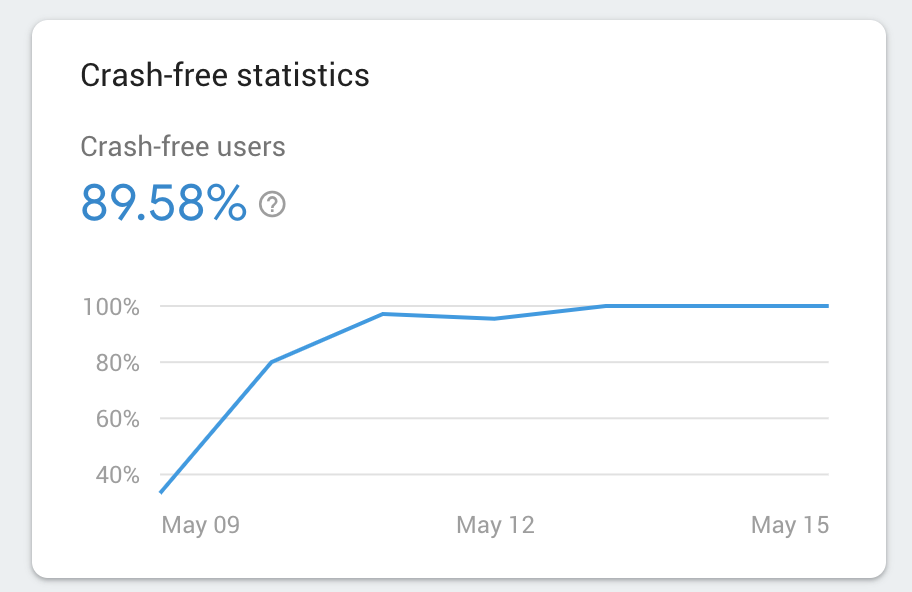
\includegraphics[scale=0.4]{analytics2}
  \caption{Crash-free user sessions}
  \label{fig:fb2}
\end{subfigure}%
\begin{subfigure}{.5\textwidth}
  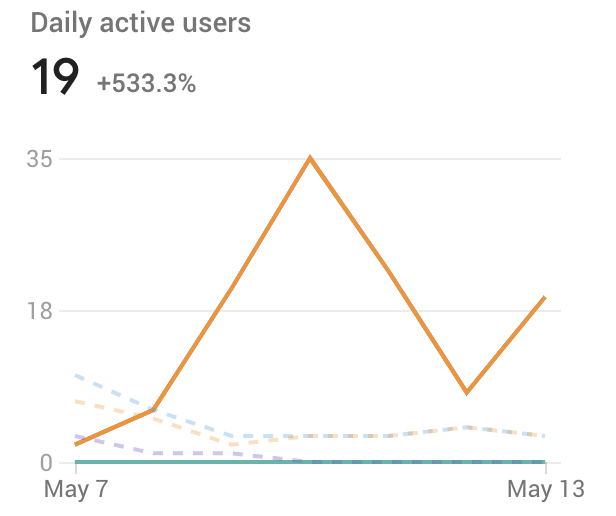
\includegraphics[scale=0.5]{analytics1}
  \caption{Daily Active Users}
  \label{fig:fb1}
\end{subfigure}
\end{figure}



\section{Usability testing}
Usability testing in software engineering is a way to see how the application is easy to use by testing it with real users. This will help to recognise "brick-walls" mentioned before so the application UX and overall design could be improved.  This step is also significant as it allows us to observe how the potential user will try to use the application.

\subsection{Preparation}
The goal of the \appname\ usability test was to test the most significant user interactions and flows. To reflect that I have created three test scenarios to cover most of the application's functionality.  Each scenario consisted of finite number of steps, with no description of how it supposed to be completed, thus simulating the actual usage of the application. The first scenario is based around content importing, collaboration and searching. The second scenario concentrates on content creation and its moderation. And the last one asks the user to find more content for his/her library and is based around learning capabilities. The whole scenario can be found in Appendix B.

Also, the post-test survey was prepared for testers to leave their feedback. The survey was needed to learn some basic information about the users like their experience with educational apps and applications in general. It also asked about the problems they have encountered during the test, which part of the test was the easiest and hard to complete and if there are some feature requests they would like share.

\subsection{The Testing Process}
Totally seven people participated in the \appname\ usability tests,  all from different age group, with different platform affiliations and four of them being students. 
The test itself was held for one user at a time.  Firstly the user was presented with a very short application description describing its core features. Next, the scenario introduction was given, and I, as an observer, was there to see how the tester have approached the task given.
After the test, the post-survey was presented for the user to fill in.

\subsection{The Test's Results}
 Library Management and all the flows related to it, such as Notebook Publishing, its sharing, notes creation and e.t.c, as well as logging in and account creation didn't raise any issues with the testers. Searching for something specific using Search Screen was also handled by all the participants. Some of the tasks, however, were revealed to be not very clear about how to complete them, and it took some time for the majority of the testers to realise how to approach it. This section describes these problems and a possible solution that could be implemented to improve the UX. 


\subsubsection{The Search Flow}


The first problem I have witnessed during the test is that for some users it was not entirely obvious how to perform the search or more specifically, where to start it. Though everyone did found the way to start it by themselves, it took some time for some testers to realise where to look. One of the testers mentioned that he would expect to see the Search Button on the application's main screen. I will monitor this problem and collect feedback from the users to determine whether or not this issue must be addressed.

\subsubsection{The Review Flow}
The functionality to review the suggestions left by the other users is very important, and the test revealed a couple of design flaws that showed the first "brick-wall" -- most of the testers were not able to complete this flow. And there multiple points to it:

\begin{itemize}
	\item{The root of all problems with this flow was the behavior of the bottom drawer that is used to confirm the changes. Most of the testers tried to click it, which is the action that was not yet. The fact that it is not clickable made them think that it is just a static element, so they gave up interacting with it.
	
	The simplest solution to this problem is to make the bottom sheet clickable, as it was the first interaction performed by a significant number of testers. Another thing that could be done is to add some elements to make the behavior a bit more obvious. This could be either an animation, arrow icon or an additional elevation.}
	\item The first problem had a significant influence on the whole process as the tester didn't know how to complete the flow. Naturally, some of the tried to leave this screen -- and the application allowed them to, even when the user had already reviewed some suggestions. This led them to think that they have completed the flow.
	
	The first thing that must be addressed is to prevent the user from immediately leaving the screen when he/she has already started the review process. This could be done using the confirmation dialog.
	
	\item{Another issue was that it was not evident for some users that the list of suggestions there is scrollable. Once the first item was reviewed, it took time for some users to realise it.
	
	
	Here the solution requires two adjustments. Firstly, to make it obvious that the screen is scrollable, it can show the preview of the next/previous element. And lastly, reviewing the suggestion could  automatically scroll to the next item in the list. This will not only reveal that the screen is scrollable but also will also handle the swipe gesture.
	}

\end{itemize}
\subsubsection{Notes Modifications}
The Notes modifications flow is core to the collaboration feature of the \appname.  After saving the Published Notebook, some of the users didn't realise what supposed to be done to create a suggestion.  This flow requires the user to navigate to the My Library screen and open the notebook they have just saved (i.e., Notes Screen). 
The solution would be to either propose to handle this navigation for them or to navigate to the saved notebook straightaway. The Notes Screen should reflect this as well, for example by adding some message to inform the user that it is possible to create a suggestion.
The solution described is not so trivial as the ones purposed before, and it will likely require more testing after its implementation.


\subsubsection{The Start of The Review Flow}
One of the steps in the scenario B described the situation of receiving the notification about new suggestion with the following step being to review this suggestion. While the interaction with notification was rather straightforward, when landing on the Published Notebook Detail Screen it took some time for the testers to find the button that will start the flow in question. 

The solution would be to re-organise this screen a bit to reflect its current state when it comes to suggestions.  Another solution to handle the notification clicks a bit more precise. Right now, no matter the notification type (New comment, new suggestion or notebook update) it will open the Published Notebook Detail Screen. While it works fine for a Notebook Update type as the user immediately sees the update button, it would make sense to open the Comments Section or the Review Screen when clicking on new comment notification and suggestion notification respectively.


\subsubsection{Results Summary}
Due to the problems described above the results are quite mixed. While it won't take too much time to address most of these issues, at least one of them requires more in-depth investigation and additional testing. On the other hand, most of the users responded that though it was not obvious how to approach the task at first when they have realised the way to do it, it became obvious for them and made sense why it's implemented the way it is. This leads to the conclusion that these kinds of problems can be addressed by adding short tutorials to onboard new users.

\setsecnumdepth{part}
\chapter{Conclusion}

The goal of this thesis was to develop a StudyPad client for Android OS, which involved domain, requirements and existing solutions analysis as the first step. Next, the application UI and architecture was designed to support the requirements established in the previous step. Finally, the application was developed applying best practices from the world of the modern Android application development.
All requirements specified in the Analysis were implemented along with the  couple new functionalities that were not a part  of the requirements specification.

Once the implementation step was completed, the application was uploaded to the Google Play Store as the part of Early Access program for beta-testing. Next the 
	usability test were performed which revealed certain problems with the initial UX implementation and ways to handle them were proposed. As for time of writing this chapter the application got 30 downloads on the Play Store, which is not a lot, but I am sure that with the incoming feedback from the existing user base and with help of other students willing to be a part of \appname\ development, the application will be discovered by a larger amount of users.
\subsection{Future development}
\appname\ development is far from over.  The current iteration of the application had an emphasis on content creation, sharing, and collaboration, with just a few tests available for users to study and learn. The real process of studying has yet to be researched and executed.
This could be a main focus for the future development of \appname.


There also some small changes that could be  addressed such as:
\begin{itemize}
	\item Powerful Notes editor that would make notes creation easier.
	\item Implementing of Paging. Currently, neither API or the Application supports paging. Paging would improve loading time, which is especially important when there is a lot of content available.
	\item Unit and Instrumentation tests to ensure application stability.
	\item Implementation of Modular Architecture. It would enhance the quality of code and make test coverage easier.
	\end{itemize}
	
	\noindent Though there are still a lot of work to be done on the Android application, \appname\ could be much bigger. In the long run, the iOS client could be finalised, and the Web client implemented making it a fully cross-platform experience. 

\bibliographystyle{iso690}
\bibliography{mybibliographyfile}


\setsecnumdepth{all}
\appendix

\chapter{Acronyms}
% \printglossaries
\begin{description}
	\item[AAC] Android Architecture Components
	\item[GUI] Graphical user interface
	\item[FIT] Faculty of Information Technology
	\item[CTU] Czech Technical University
	\item[BI-EJA] Enterprise Java
	\item[BI-AND] Programming for the Android Operating System
	\item[BI-IOS] Fundamentals of iOS Application Development for iPhone and iPad
	\item[BI-SP1] Team Software Project 1
	\item[BI-SP2] Team Software Project 2
	\item[XML] Extensible markup language
	\item[FAB] Floating Action Button
	\item[UI] User Interface
	\item[UX] User Experience
	\item[FCM] Firebase Messaging Service
	\item[GCM] Google Messaging Service
	\item[DSL] Domain Specific Language
	\item[DI] Dependency Injection
	\item[IoC] Inversion of Control
\end{description}



\chapter{Testing Scenarios}

\section{Scenario A}
\begin{enumerate}
	\item Login using following credentials: test2@studypad.com  12345678
	\item Notice that you don't have any notebooks saved
	\item You'd like to learn Czech language.
	\item Open Search Screen.
	\item Find all notebooks relevant your category.
	\item Select the notebook named Czech Me and import it to you library.	
	\item Open through notebook you've just saved.
	\item  Notice that some data inside looks wrong or incomplete.
	\item Choose two notes and modify them
	\item Add new note with some content.
	\item Open published version of this notebook and make a suggestion.
	\item Leave a comment and delete the notebook from you library.



	 

\end{enumerate}

\section{Scenario B}

\begin{enumerate}
	\item Login using following credentials: test1@studypad.com  12345678.
	\item  Notice that you have some unread notifications -- someone  have just asked to to update one of your notebooks.
	\item  Look through the changes made.
	\item  Find the changes your changes and approve them, reject 1 change from user named Buggy Jack
	\item  You'd like to create more study materials and share them with others.
	\item  Create new notebook.
	\item  Create a couple of notes inside.
	\item  Publish this notebook.
	\item Make some changes to a notes and update the published version.
	\item Share the link to this notebook with someone.
\end{enumerate}

   
   
\section{Scenario C}

\begin{enumerate}
	\item You'd like to recall your high school program.
	\item  Find notebooks from related to  algebra.
	\item  Explore the results, choose one and save it.
	\item  Explore the notebooks, choose one and save it.
	\item  Start one of the challenges using this notebook and complete it
	\item  Find the changes your changes and approve them, reject 1 change from user named Buggy Jack
\end{enumerate}




\chapter{Contents of enclosed CD}


%change appropriately

\begin{figure}
	\dirtree{%
		.1 readme.txt\DTcomment{the file with CD contents description}.
		.1 studypad.apk\DTcomment{Android installation file}.
		.1 BP\_Levinzon\_Roman\_2019.pdf\DTcomment{the thesis text in PDF format}.
		.1 src\DTcomment{the directory of source codes}.
		.2 studypad-android\DTcomment{android app source code}.
		.2 studypad.mdj\DTcomment{StarUML diagrams source}.
		.2 studypad.sketch\DTcomment{Sketch source file}.
		.2 studypad-thesis\DTcomment{the directory of \LaTeX{} source codes of the thesis}.
		.1 attachments.
		.2 documentation\DTcomment{android app javadoc}.
		.2 survey\DTcomment{Test survey and its results}.
		}
	\end{figure}
\end{document}
